\section{Программная реализация}

\subsection{Предобработка данных}

Прежде чем приступить к построению и обучению любой интеллектуальной системы — будь то нейронная сеть, нечеткая система или гибридный метод — критически важно убедиться в качестве и корректности входных данных. Современные алгоритмы машинного обучения крайне чувствительны к шуму, выбросам, разным масштабам признаков и пропускам, поэтому этап предобработки часто определяет успешность всей работы.

В качестве демонстрационного примера я использовал классический набор данных Iris\footnote{Fisher R.A. (1936). \emph{The use of multiple measurements in taxonomic problems}. Annals of Eugenics, 7(2):179–188.}. Этот набор содержит 150 образцов ирисов трёх видов (\emph{Iris setosa}, \emph{Versicolor}, \emph{Virginica}), описанных четырьмя числовыми признаками:
\begin{itemize}
  \item длина чашелистика (sepal length), см;
  \item ширина чашелистика (sepal width), см;
  \item длина лепестка (petal length), см;
  \item ширина лепестка (petal width), см.
\end{itemize}
Каждому образцу сопоставлен целевой класс — один из трёх видов ириса.

\medskip
\noindent\textbf{Основные этапы предобработки данных:}
\begin{enumerate}
  \item \textbf{Первичный анализ}  
    \begin{itemize}
      \item Проверка отсутствующих значений и аномалий.
      \item Вычисление базовых статистик (среднее, стандартное отклонение, квартили).
      \item Визуализация распределений (гистограммы) и парных зависимостей (scatter–matrix).
    \end{itemize}
  \item \textbf{Выявление и удаление выбросов}  
    С помощью межквартильного метода и визуальных средств (ящика с усами) отмечаются экстремальные значения, которые могут искажать обучение.
  \item \textbf{Нормализация и масштабирование}  
    Для равномерного вклада всех признаков используется стандартизация (z-score) или min–max нормализация:
    \[
      x' = \frac{x - \mu}{\sigma},\quad
      x'' = \frac{x - x_{\min}}{x_{\max}-x_{\min}}.
    \]
  \item \textbf{Разбиение на обучающую и тестовую выборки}  
    Обычно данные делятся в соотношении 70\%–30\% или 80\%–20\%, с последующим стратифицированным отбором образцов, чтобы сохранить пропорции классов.
\end{enumerate}

\subsection{Инструменты анализа}

Для качественной предобработки и первичной оценки данных используются следующие ключевые приёмы визуализации:

\begin{description}
  \item[Гистограмма (Histogram)]  
    \hfill 
    \begin{itemize}
      \item \textbf{Назначение:} 
        
        оценить форму распределения одного числового признака, выявить асимметрию, мультимодальность и выбросы.
      \item \textbf{Как читать:} 
        
        по горизонтали — интервалы значений (бины), по вертикали — количество образцов.  
      \item \textbf{Рекомендации:}  
        \begin{itemize}
          \item Подберите число бинов так, чтобы не терялось основное «полотно» распределения, но и не было слишком «рвано».  
          \item Обратите внимание на пики — возможные подгруппы данных.  
          \item Узкие «хвосты» помогут заметить редкие выбросы.
        \end{itemize} 
    \end{itemize}

  \item[Boxplot–диаграмма (Box–Whisker)]  
    \hfill
    \begin{itemize}
      \item \textbf{Назначение:} 
        
        сравнить распределения одного признака между группами (видами iris), одновременно увидеть медиану, квартильные границы и выбросы.
      \item \textbf{Как читать:}  
        \begin{itemize}
          \item Ящик (box) — межквартильный интервал (Q1–Q3), линия внутри — медиана.  
          \item Усы (whiskers) — выборочные границы (обычно $Q1-1.5 \cdot IQR, Q3+1.5 \cdot IQR$).  
          \item Точки за усами — выбросы.
        \end{itemize}
      \item \textbf{Рекомендации:}  
        \begin{itemize}
          \item Сравнивайте положения медиан для разных групп.  
          \item Используйте одну палитру для согласованности.  
          \item При разметке терминов в нечеткой системе берите Q1, Q2, Q3 как опорные точки.
        \end{itemize}
    \end{itemize}

  \item[Матрица рассеяния (Scatter–matrix)]  
    \hfill
    \begin{itemize}
      \item \textbf{Назначение:} 
        
        одновременно визуализировать попарные зависимости и распределения всех признаков.
      \item \textbf{Как читать:}  
        \begin{itemize}
          \item Диагональные ячейки — гистограммы каждого признака.  
          \item Вне диагонали — точечные диаграммы (scatter plots) для пары признаков.
        \end{itemize}
      \item \textbf{Рекомендации:}  
        \begin{itemize}
          \item Ищите пары с минимальным перекрытием классов — эти сочетания наиболее информативны для классификатора.  
          \item Линейная или кластераная структура подскажет, что выбирать в качестве antecedent–признаков.
        \end{itemize}
    \end{itemize}

  \item[K–Means кластеризация (Cluster Plot)]  
    \hfill
    \begin{itemize}
      \item \textbf{Назначение:} быстро оценить естественную группировку данных в выбранном признаковом пространстве.
      \item \textbf{Как читать:}  
        \begin{itemize}
          \item Точки раскрашены по присвоенному кластеру.  
          \item Центроиды отображаются метками (крестиками).  
          \item Легенда и подписи кластеров помогают связать группы с реальными классами.
        \end{itemize}
      \item \textbf{Рекомендации:}  
        \begin{itemize}
          \item Используйте кластер-плот для предпосева числа терминов в нечеткой системе.  
          \item Оценивайте степень «смешивания» точек разных классов внутри одного кластера.  
          \item Корректируйте число кластеров ($k$) и наблюдайте устойчивость центроидов.
        \end{itemize}
    \end{itemize}
\end{description}

\subsection{Анализ исходных данных (Iris Dataset)}


Прежде чем приступать к построению нечеткой сети, необходимо тщательно изучить и подготовить исходный датасет. В качестве демонстрационного примера мы используем классический набор \emph{Iris} (150 образцов, 4 числовых признака, 3 класса).

\subsubsection{Статистическое описание}
\begin{table}[H]
  \centering
  \caption{Базовые статистические характеристики признаков Iris Dataset.}
  \begin{tabular}{lrrrr}
    \toprule
    Признак & Среднее & СКО & Мин. & Макс. \\
    \midrule
    sepal length (cm) & 5.84 & 0.83 & 4.30 & 7.90 \\
    sepal width  (cm) & 3.06 & 0.44 & 2.00 & 4.40 \\
    petal length (cm) & 3.76 & 1.77 & 1.00 & 6.90 \\
    petal width  (cm) & 1.20 & 0.76 & 0.10 & 2.50 \\
    \bottomrule
  \end{tabular}
  \label{tab:iris_stats}
\end{table}

\subsubsection{Распределение признаков}

На рис.~\ref{fig:iris_histos} представлены гистограммы всех четырёх признаков, построенные с цветовой палитрой.
\begin{figure}[H]
  \centering
  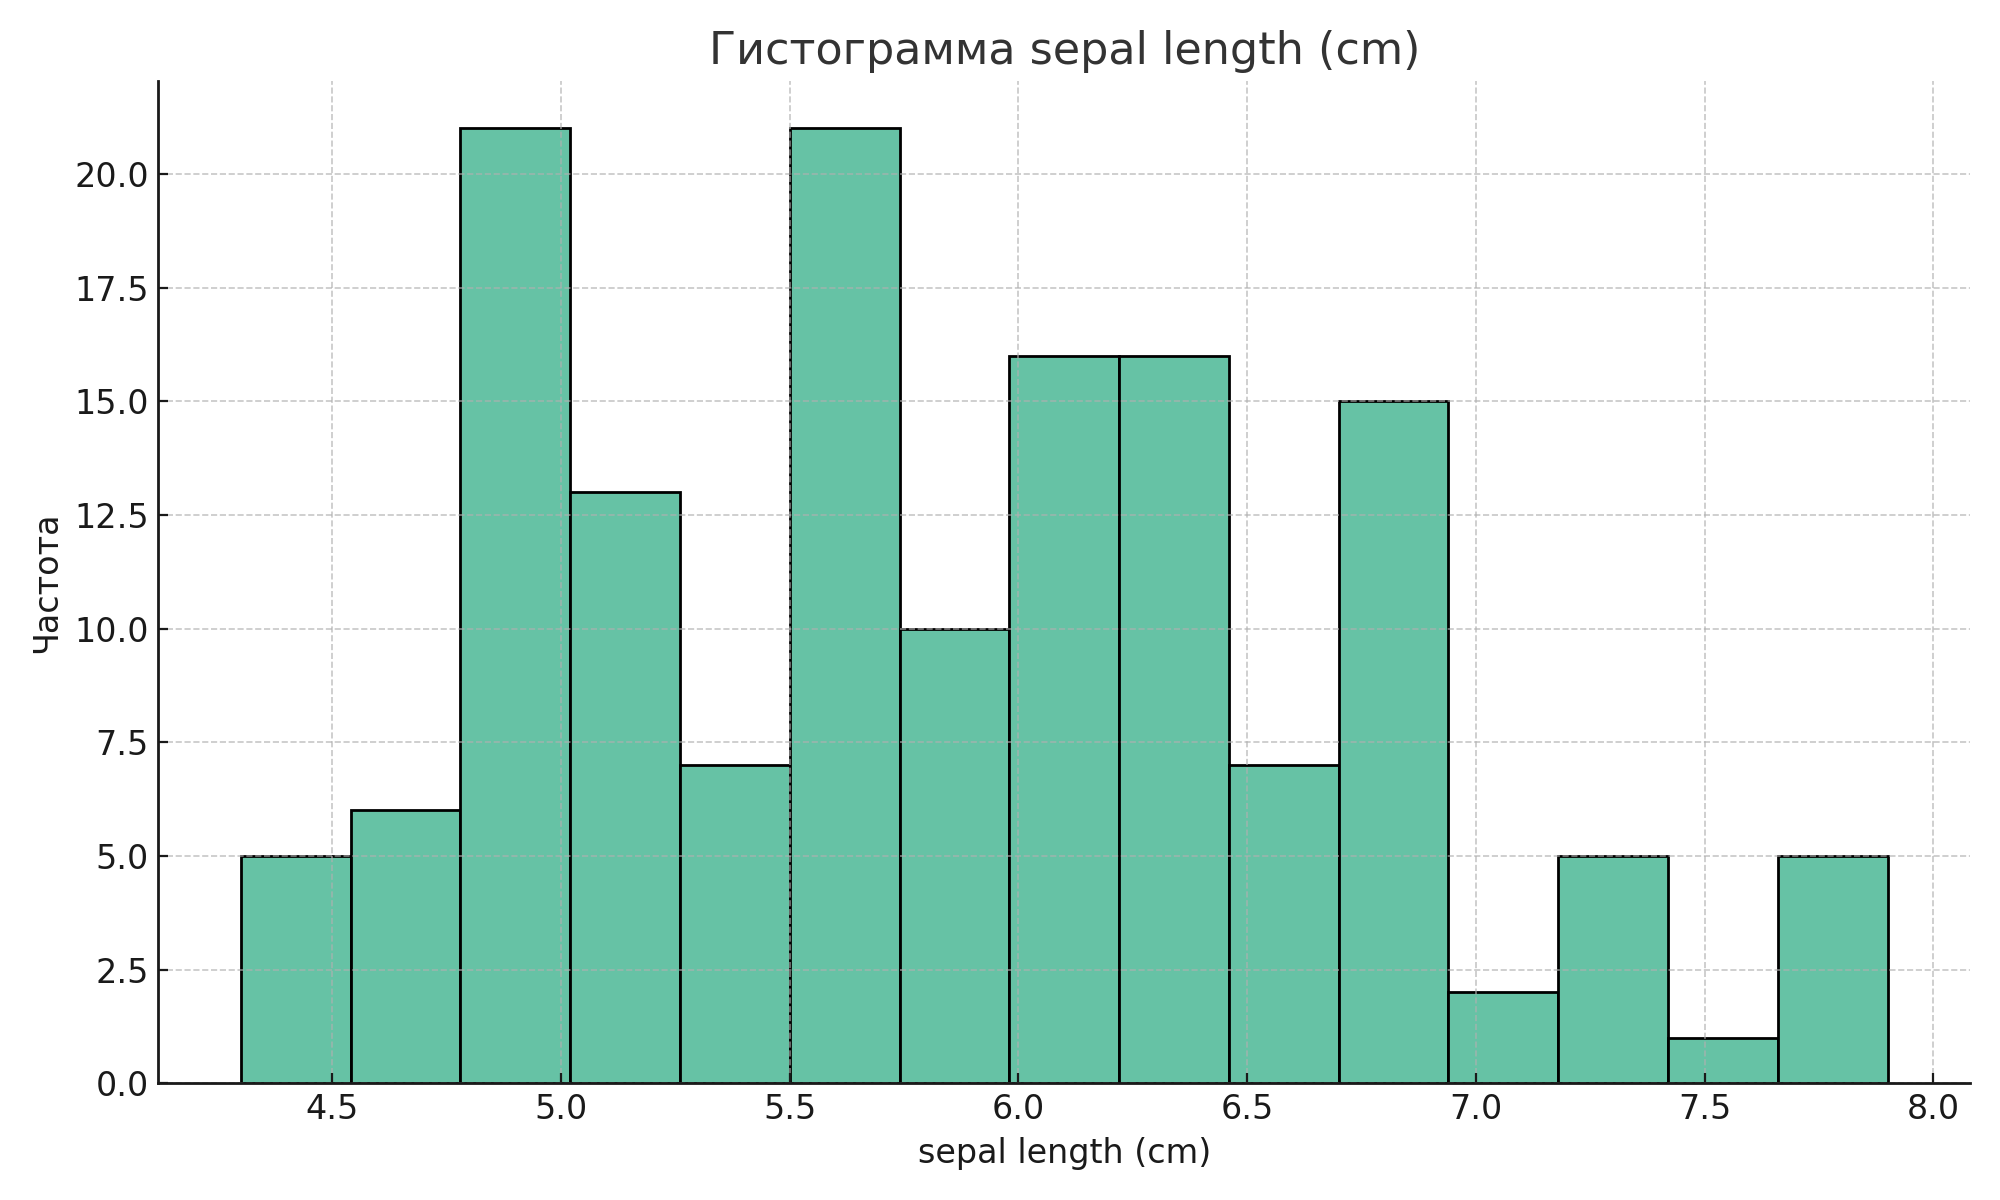
\includegraphics[width=0.8\textwidth]{images/histo_sepal_length_cm_cb2.png}\\[6pt]
  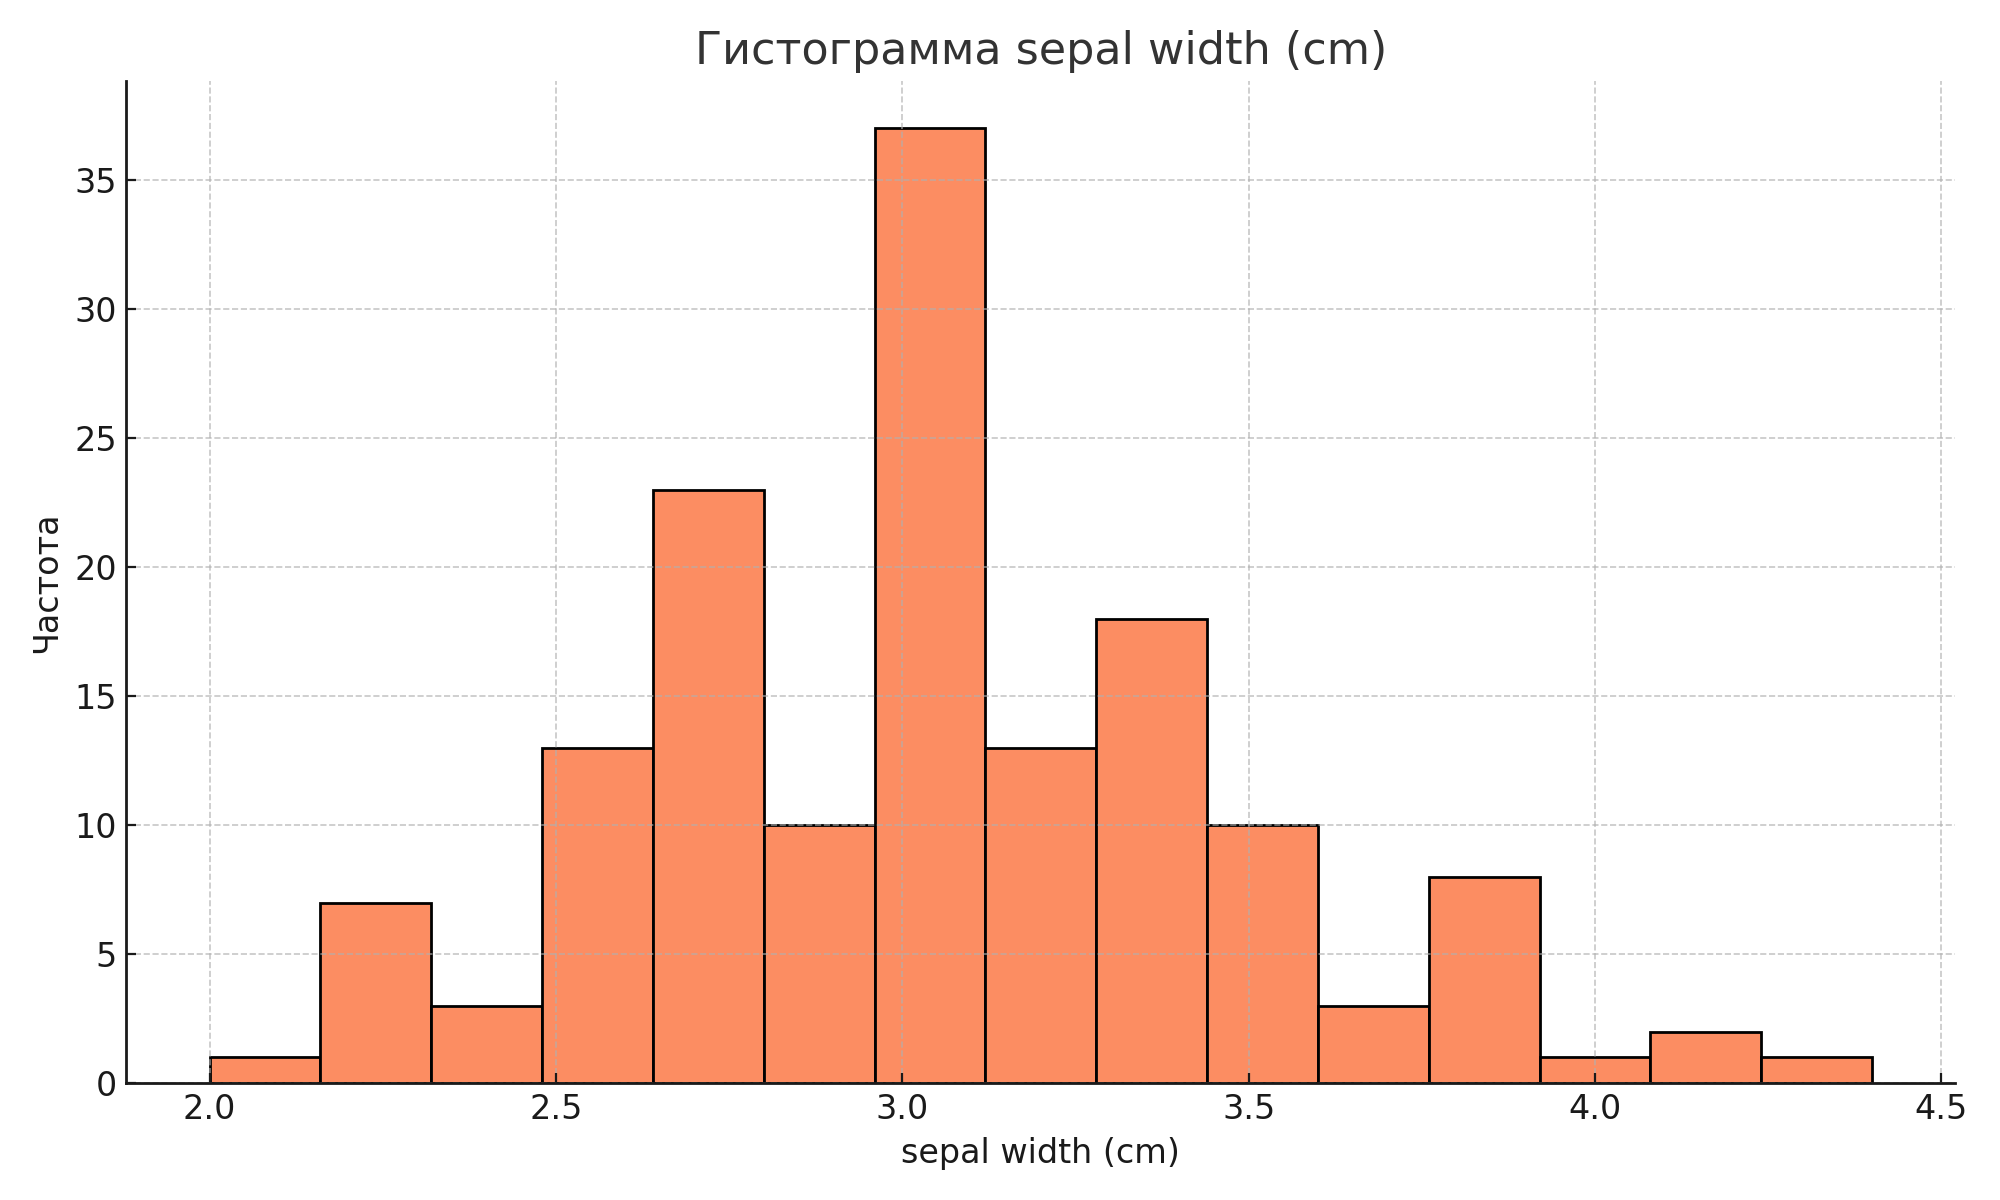
\includegraphics[width=0.8\textwidth]{images/histo_sepal_width_cm_cb2.png}
  \caption{Гистограммы распределений признаков Iris Dataset.}
  \label{fig:iris_histos}
\end{figure}

\begin{figure}[H]\ContinuedFloat
  \centering
  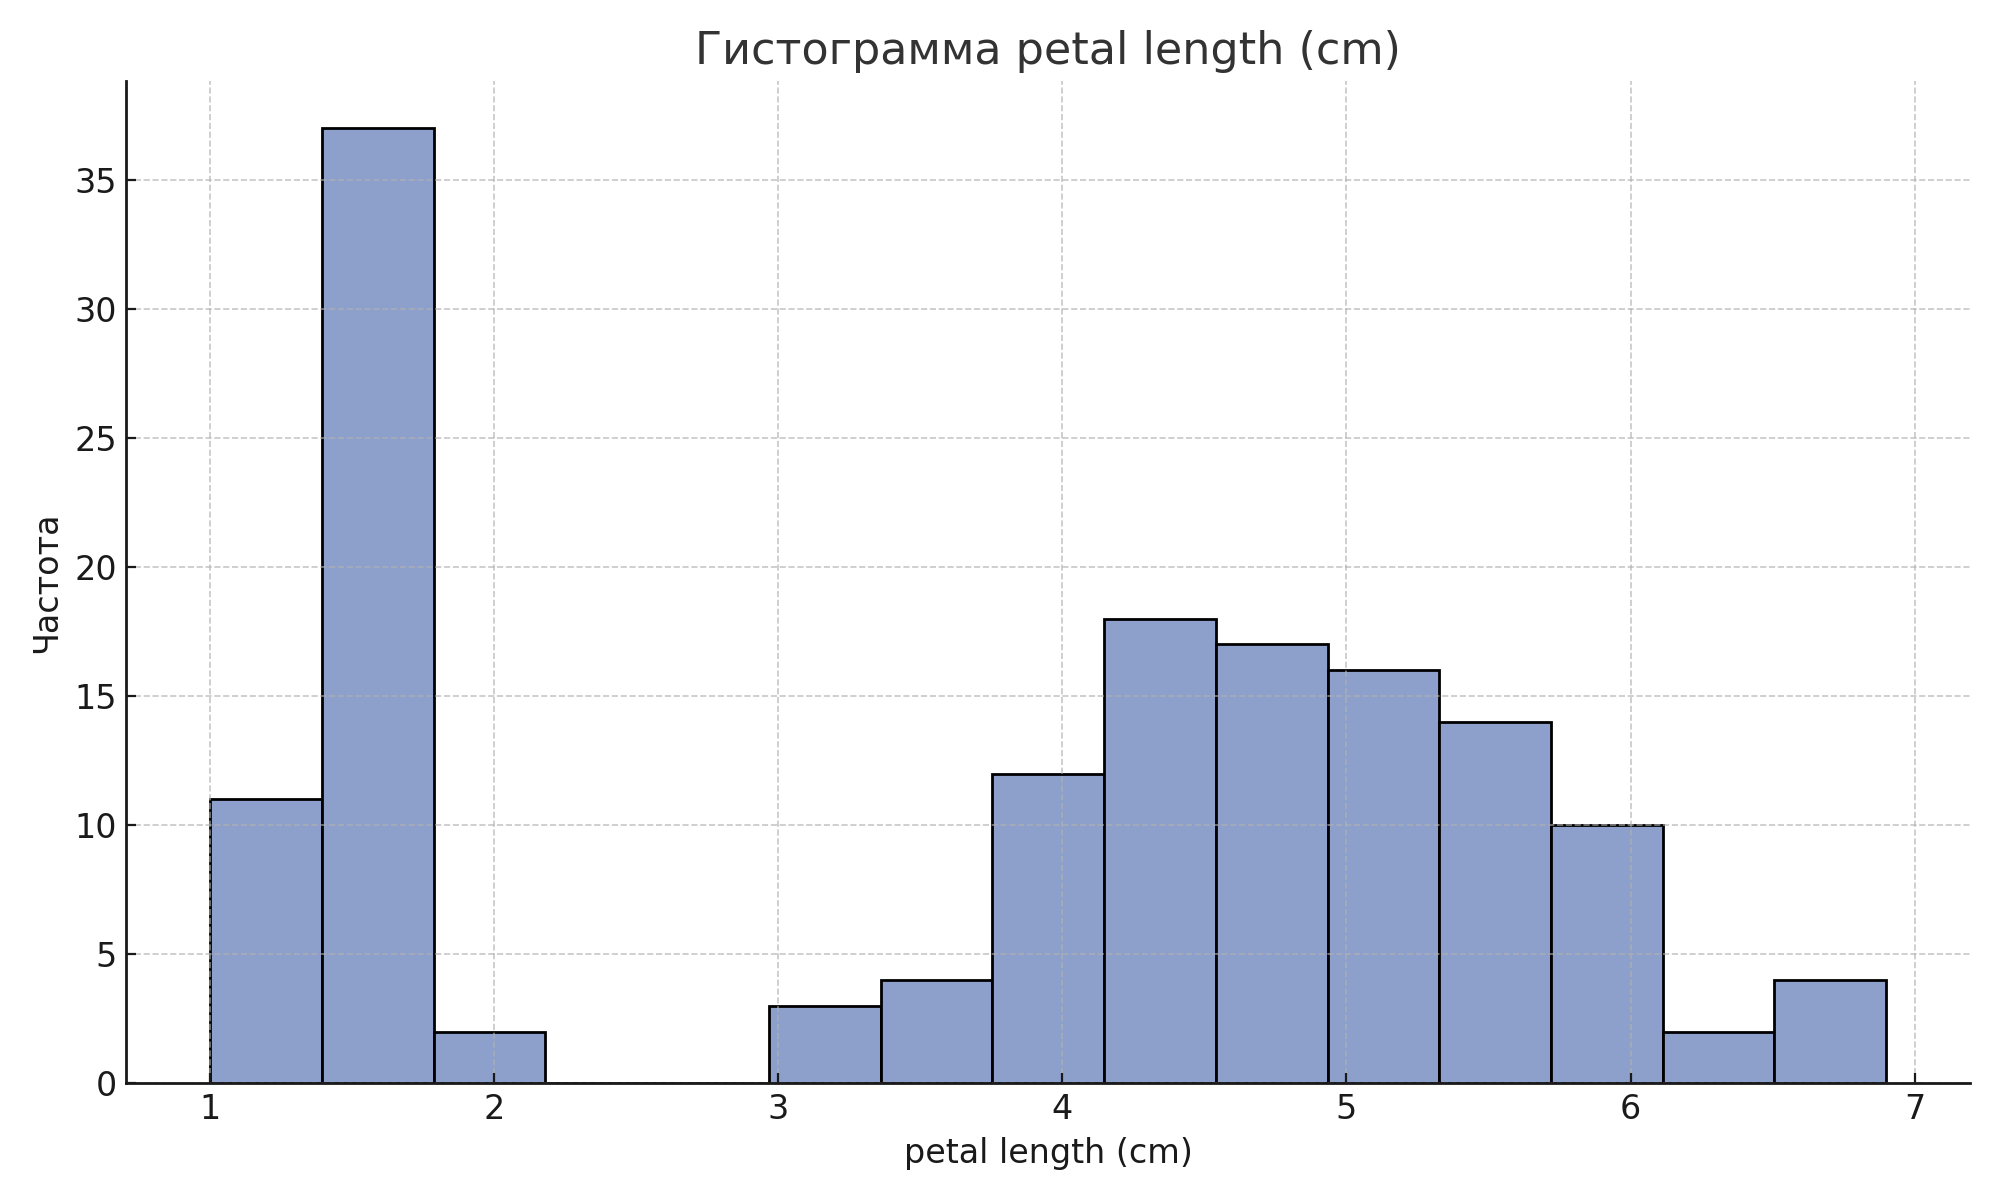
\includegraphics[width=0.8\textwidth]{images/histo_petal_length_cm_cb2.png}\\[6pt]
  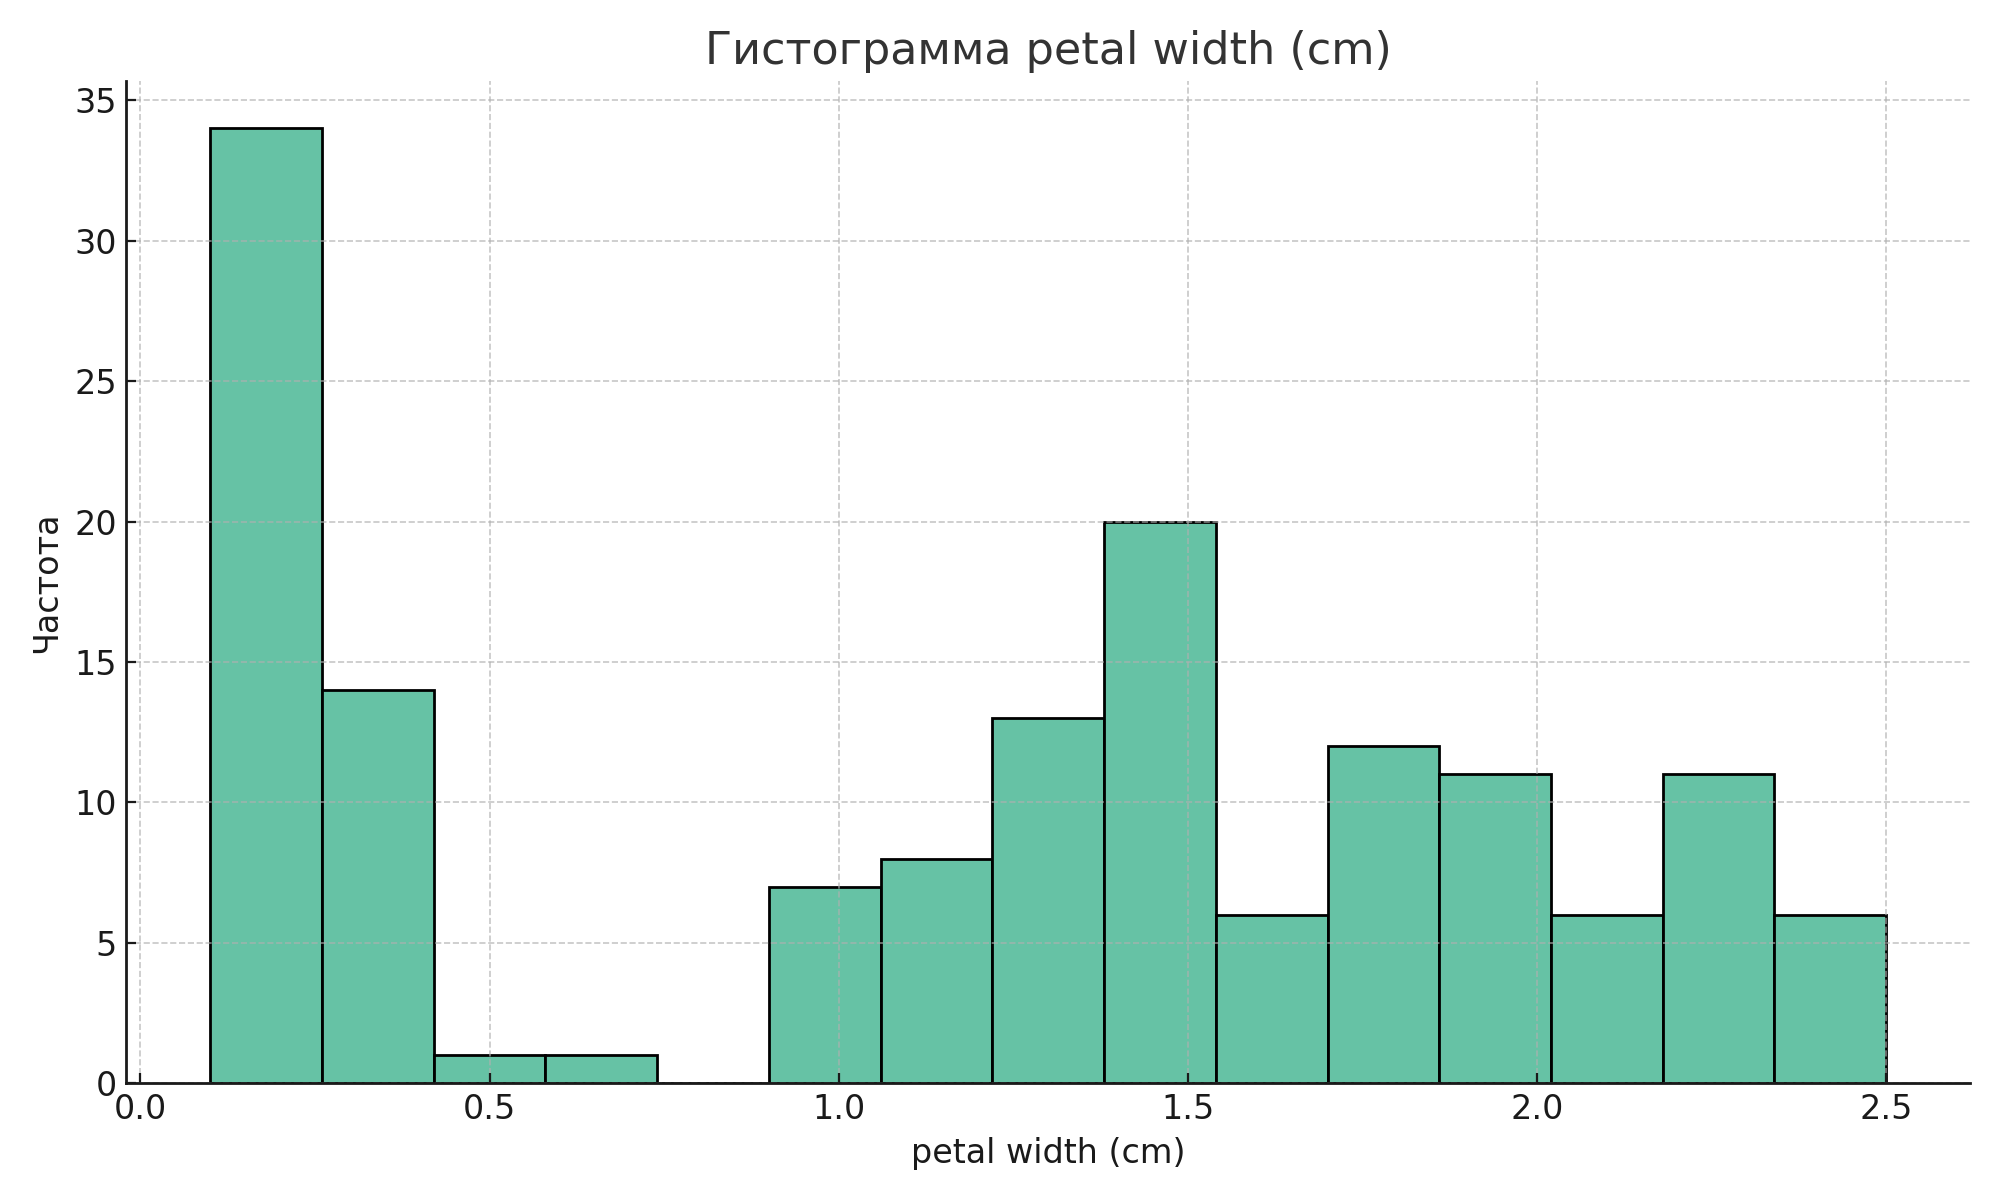
\includegraphics[width=0.8\textwidth]{images/histo_petal_width_cm_cb2.png}
  % не вызываем \caption — подпись продолжится от предыдущего блока
\end{figure}

\paragraph{Выводы.}
\begin{itemize}
  \item \textbf{sepal length} демонстрирует почти нормальное распределение с лёгкой дву­пиковостью (Setosa vs.~остальные виды).
  \item \textbf{sepal width} скошено вправо, большинство значений в [2.5, 3.5] см.
  \item \textbf{petal length} и \textbf{petal width} отчётливо мультимодальны: Setosa образует узкий «низ» (1–2 см), Versicolor и Virginica смещены вправо.
\end{itemize}

\subsubsection{Boxplot–анализ по видам}

Распределения по классам показаны на рис.~\ref{fig:iris_boxplots_vertical}.
\begin{figure}[H]
  \centering
  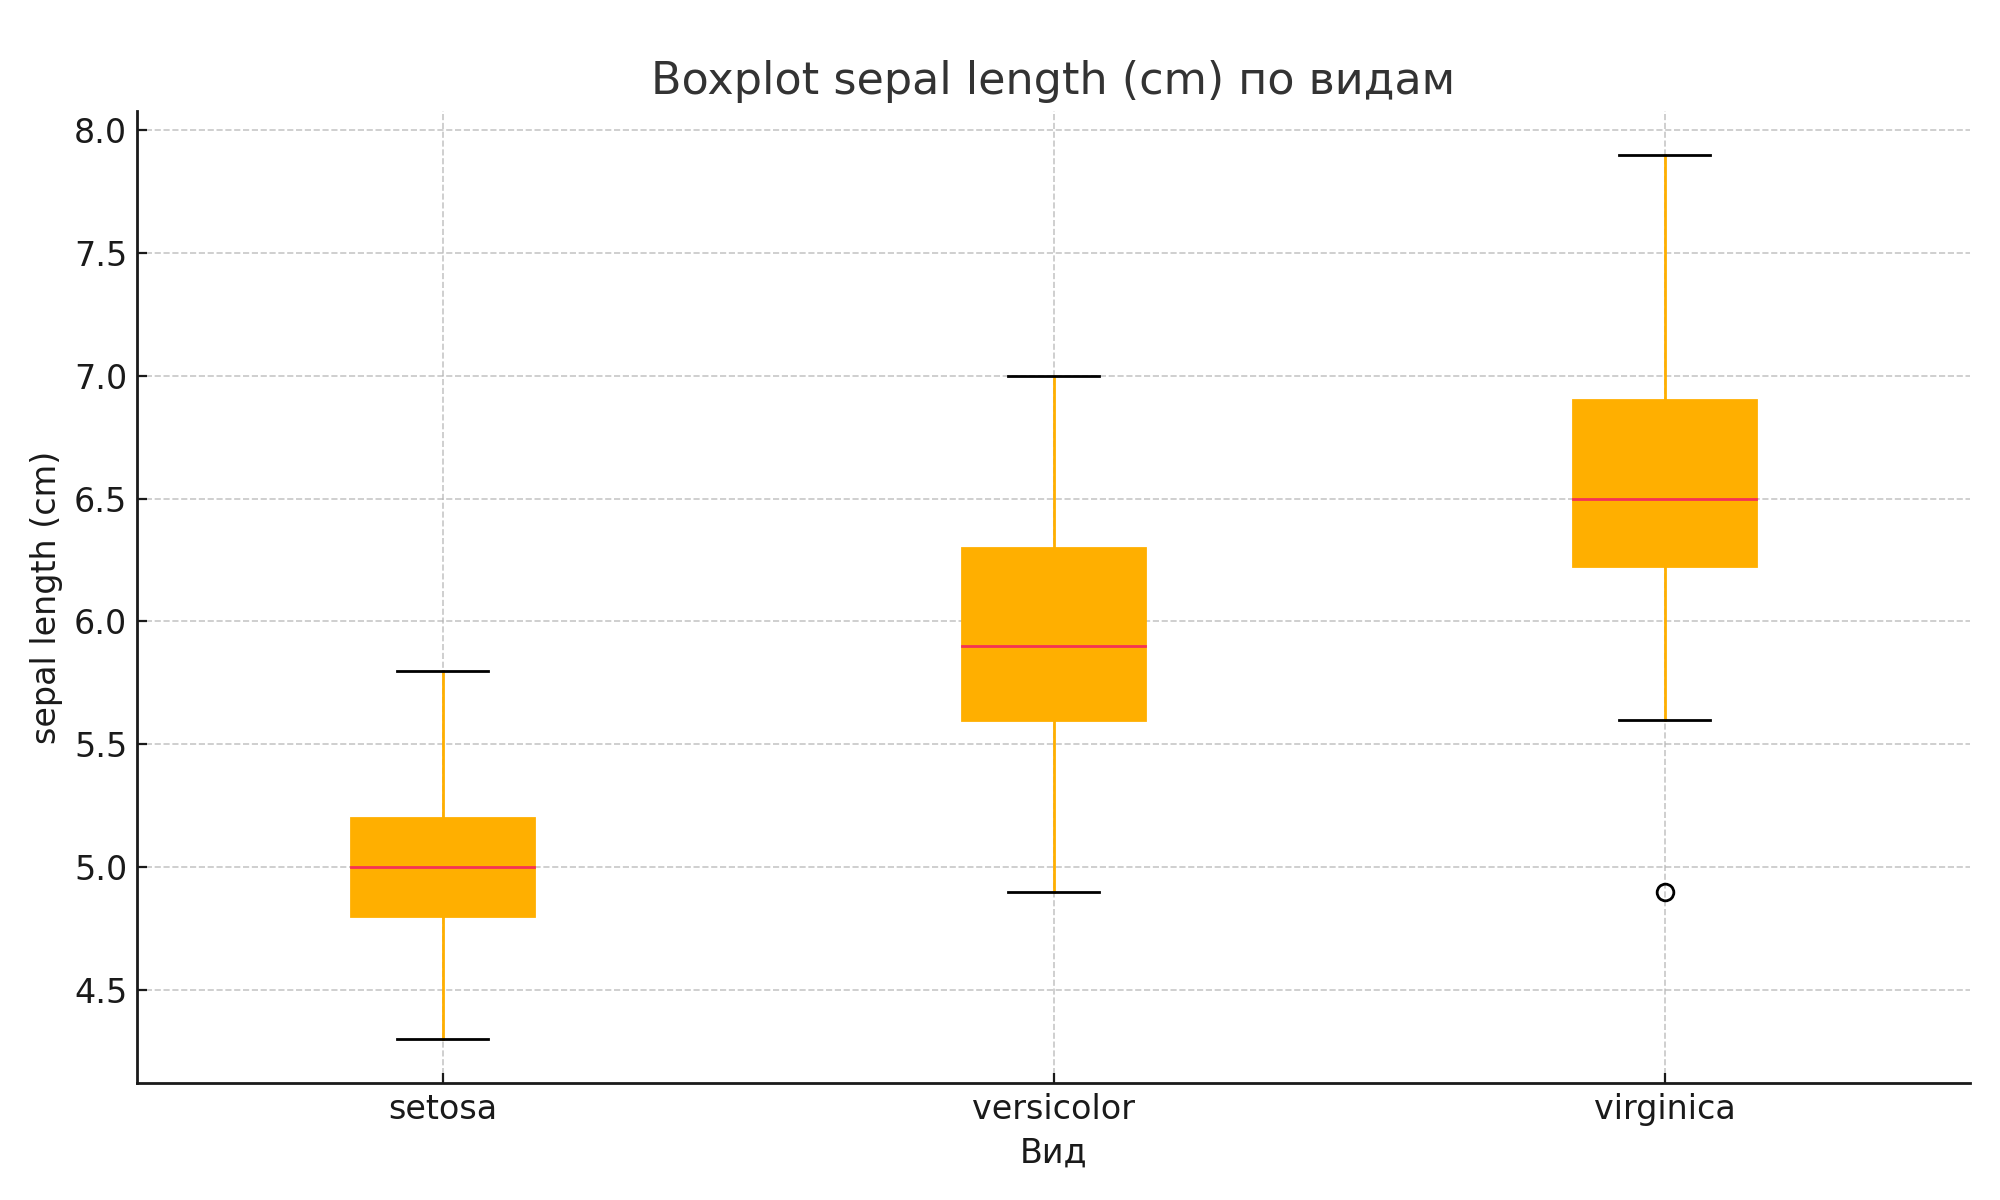
\includegraphics[width=0.8\textwidth]{images/box_sepal_length_cm_cb2.png}\\[6pt]
  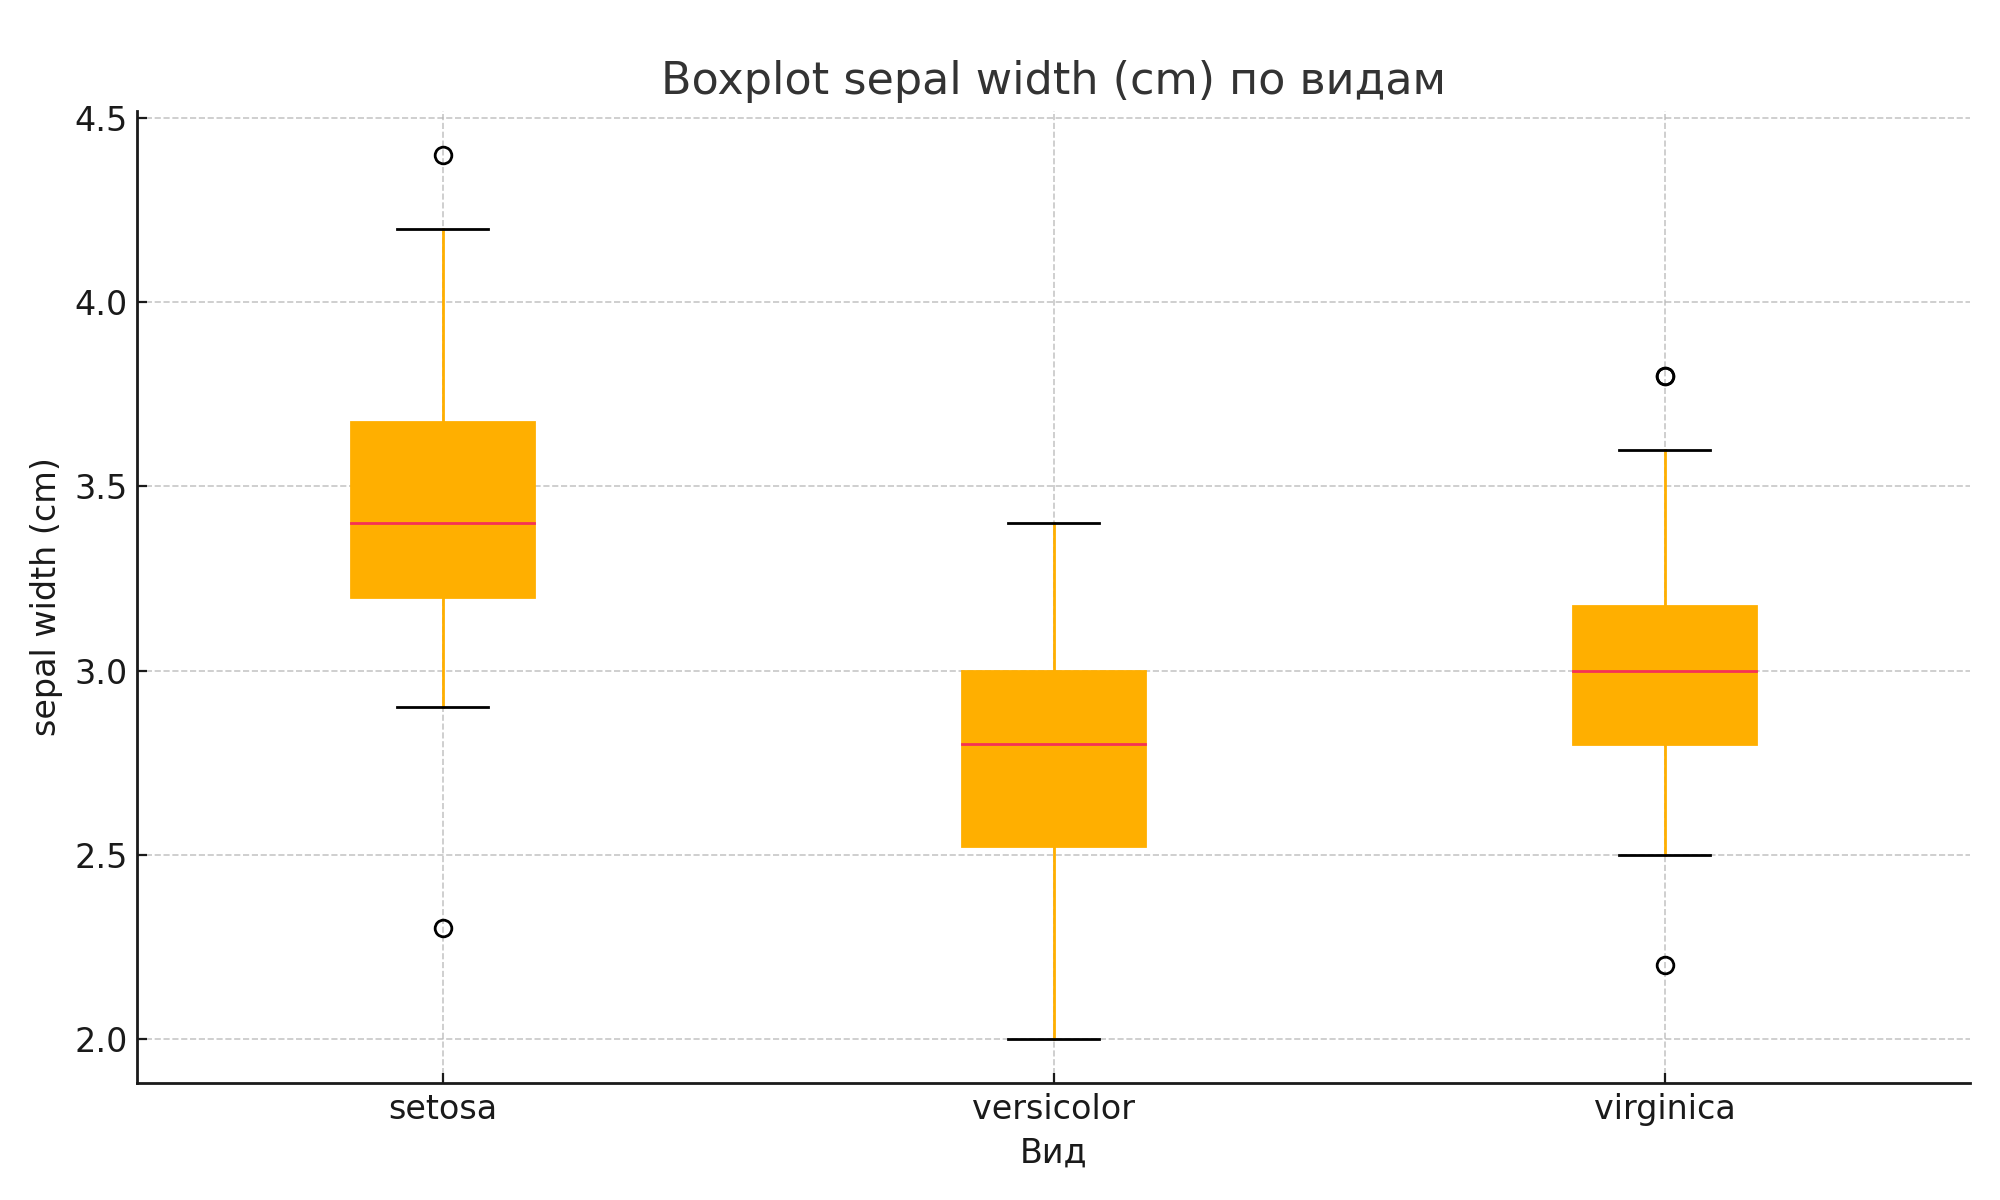
\includegraphics[width=0.8\textwidth]{images/box_sepal_width_cm_cb2.png}
  \caption{Boxplot–диаграммы признаков по видам Iris Dataset.}
  \label{fig:iris_boxplots_vertical}
\end{figure}

\begin{figure}[H]
  \ContinuedFloat
  \centering
  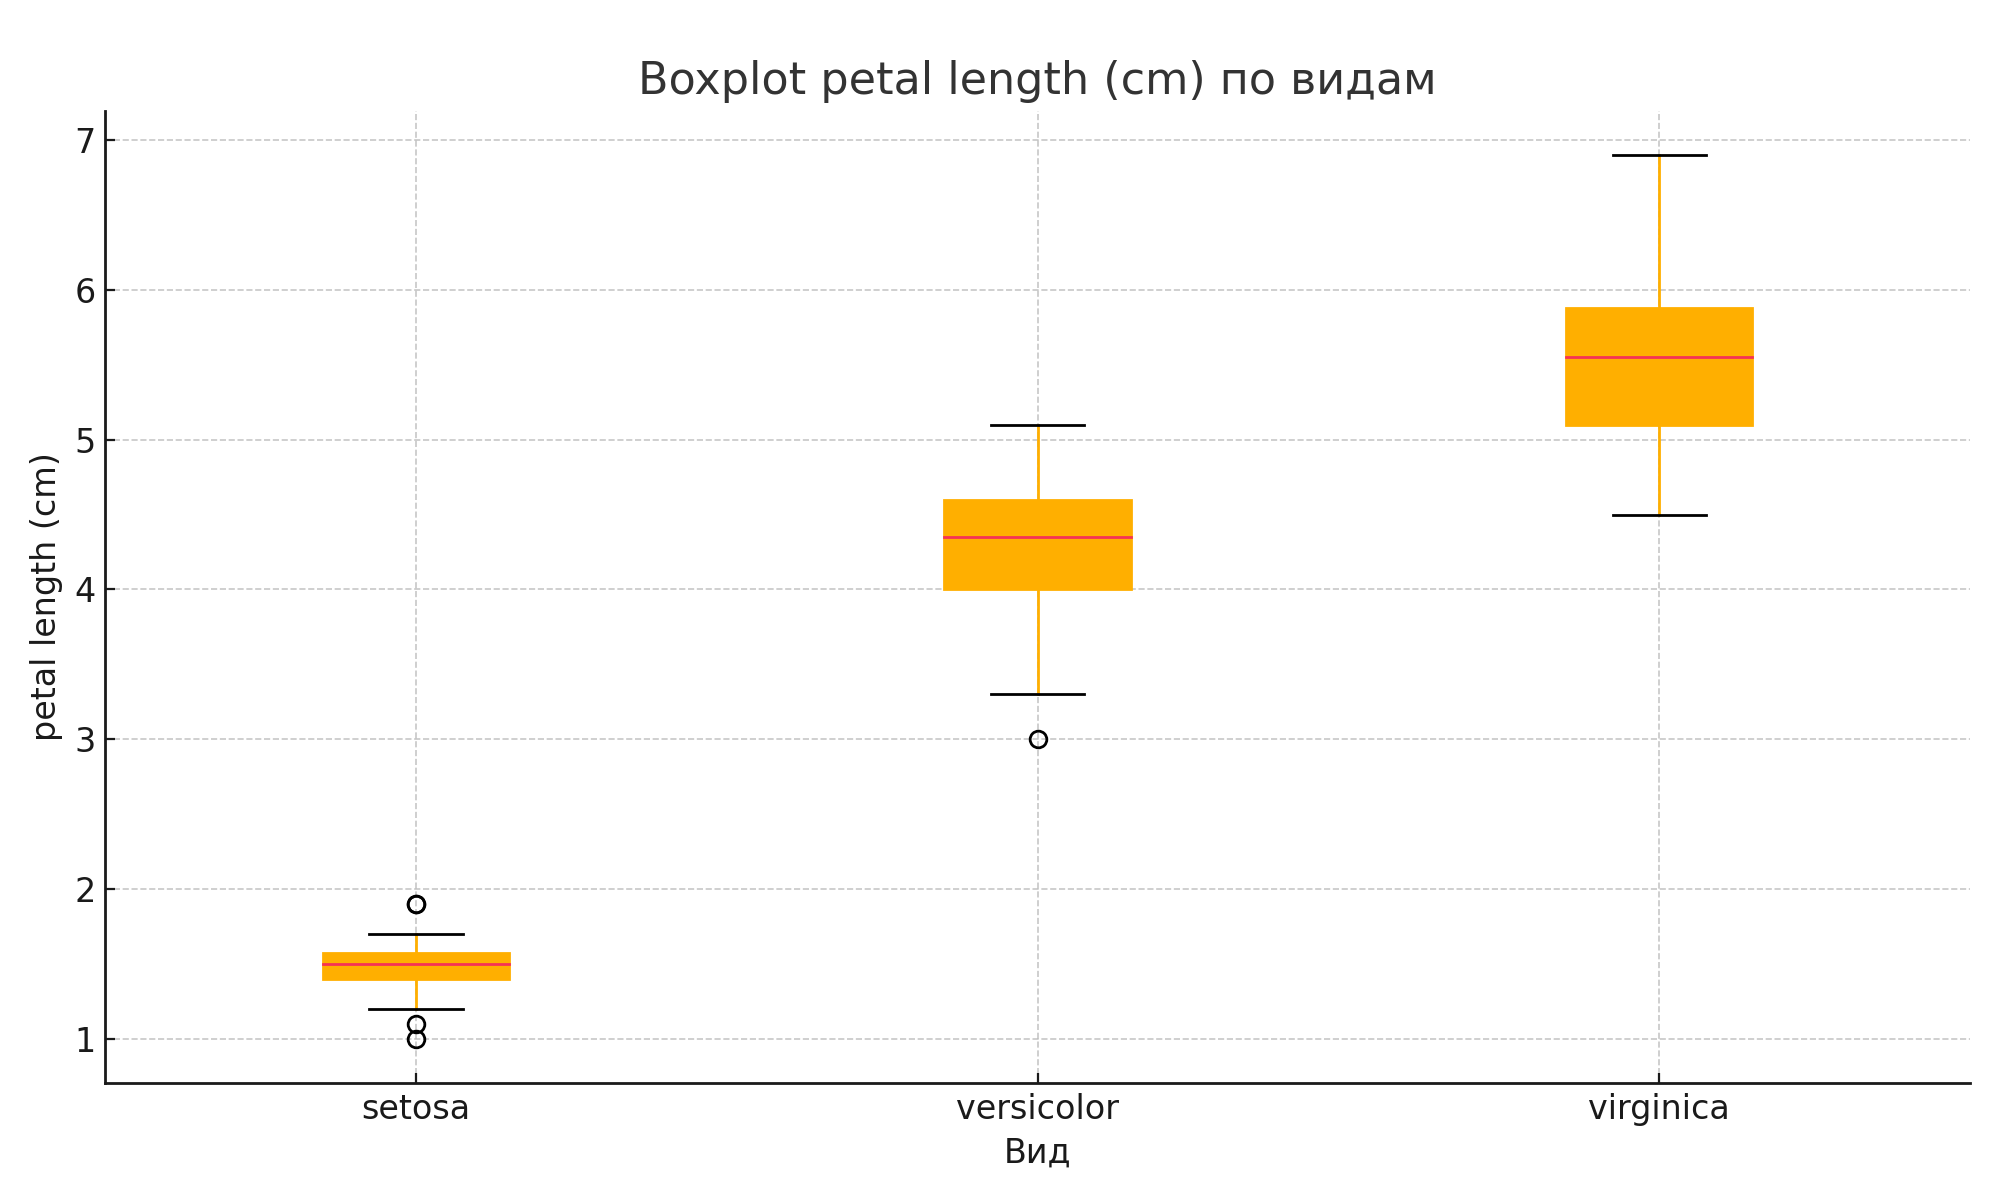
\includegraphics[width=0.8\textwidth]{images/box_petal_length_cm_cb2.png}\\[6pt]
  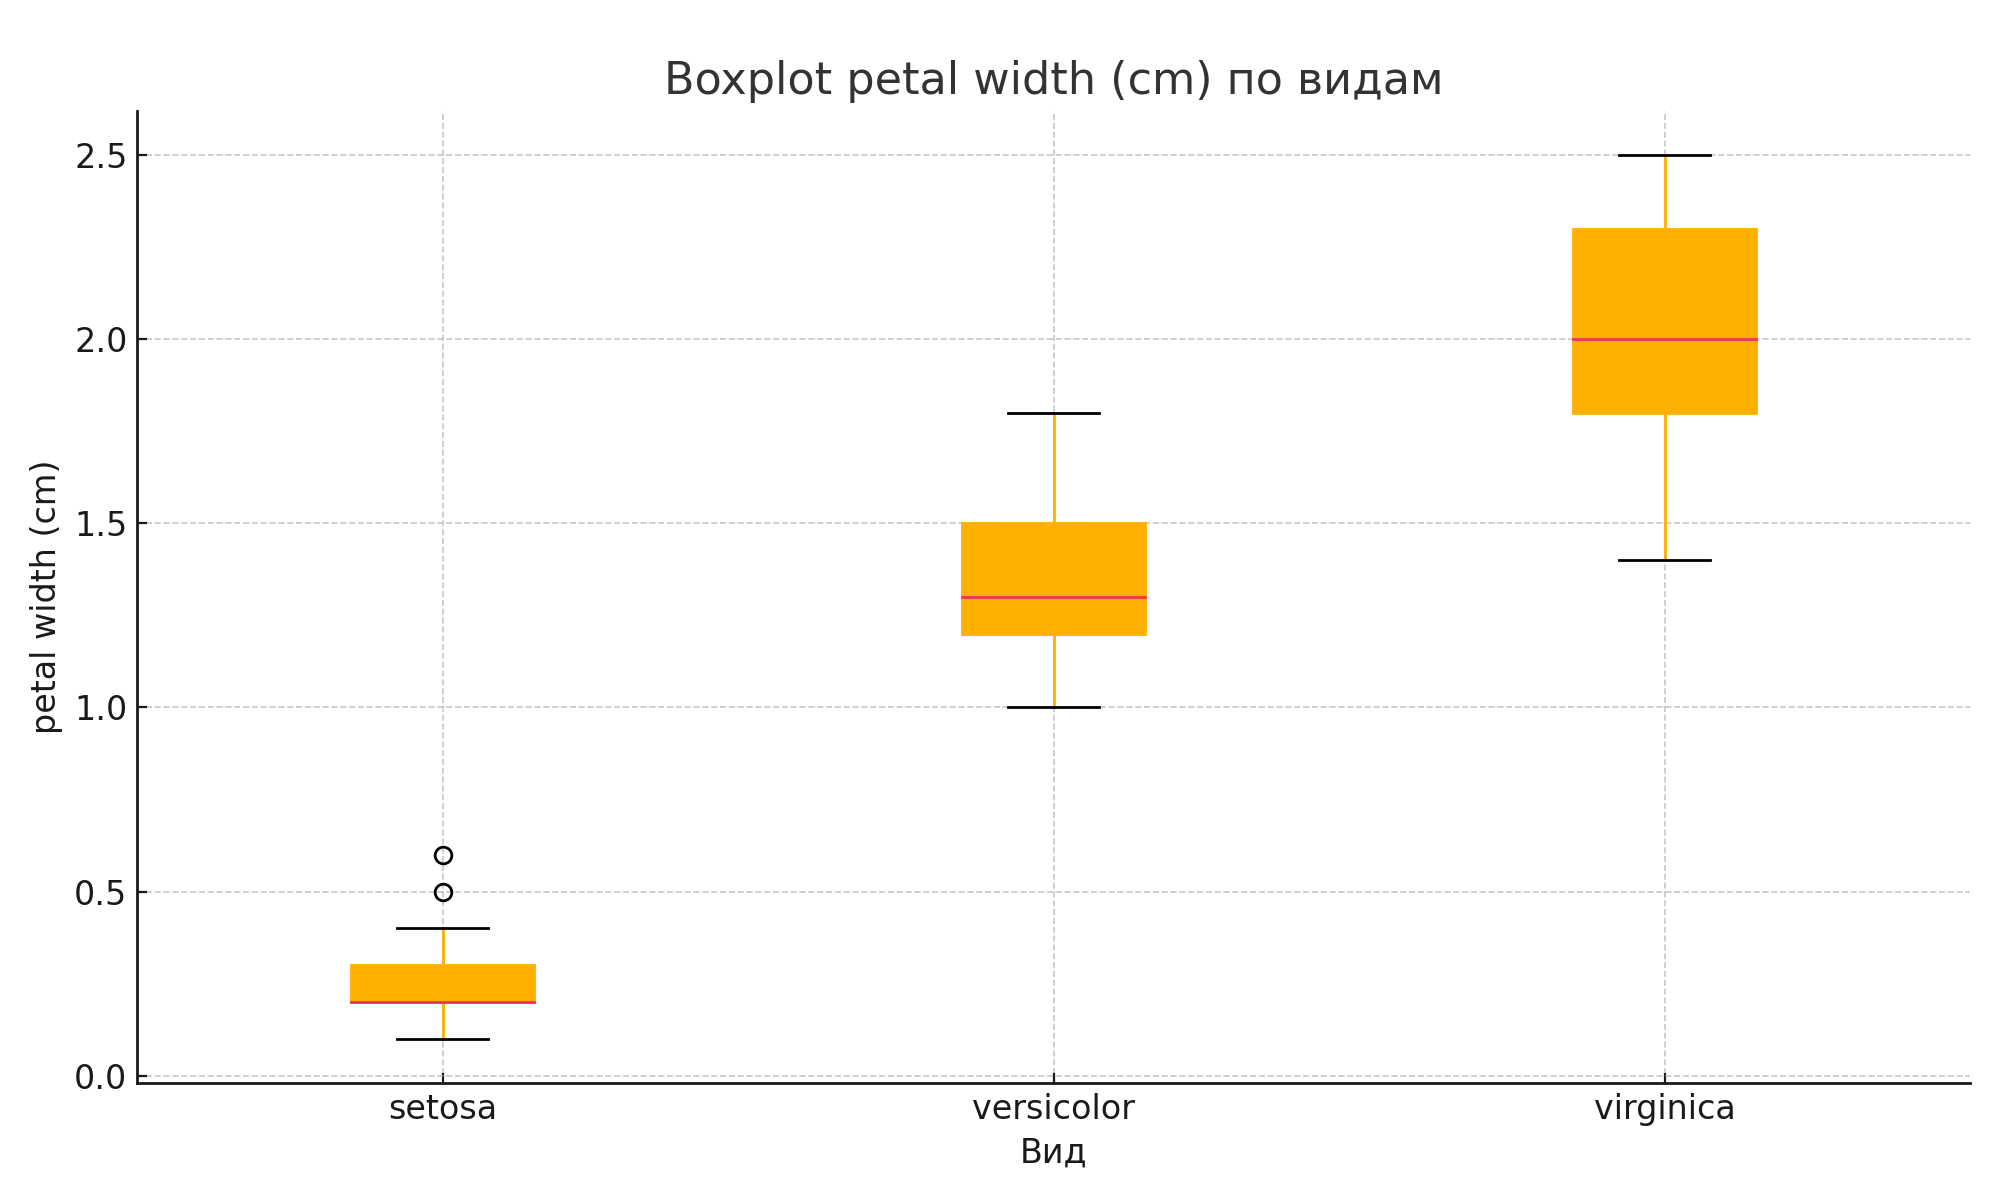
\includegraphics[width=0.8\textwidth]{images/box_petal_width_cm_cb2.png}
  \caption{Boxplot–диаграммы признаков по видам Iris Dataset.}
\end{figure}

\paragraph{Выводы.}
\begin{itemize}
  \item Для \emph{petal length/width} квартильные интервалы видов не перекрываются → признаки почти идеальны для классификации.
  \item Для \emph{sepal length/width} наблюдаются пересечения квартилей Versicolor и Virginica, поэтому они менее информативны в отрыве от лепестковых.
\end{itemize}

\subsubsection{Парная визуализация (Scatter–matrix)}

На рис.~\ref{fig:scatter_matrix} приведена матрица рассеяния всех пар признаков.

\begin{figure}[ht]
  \centering
  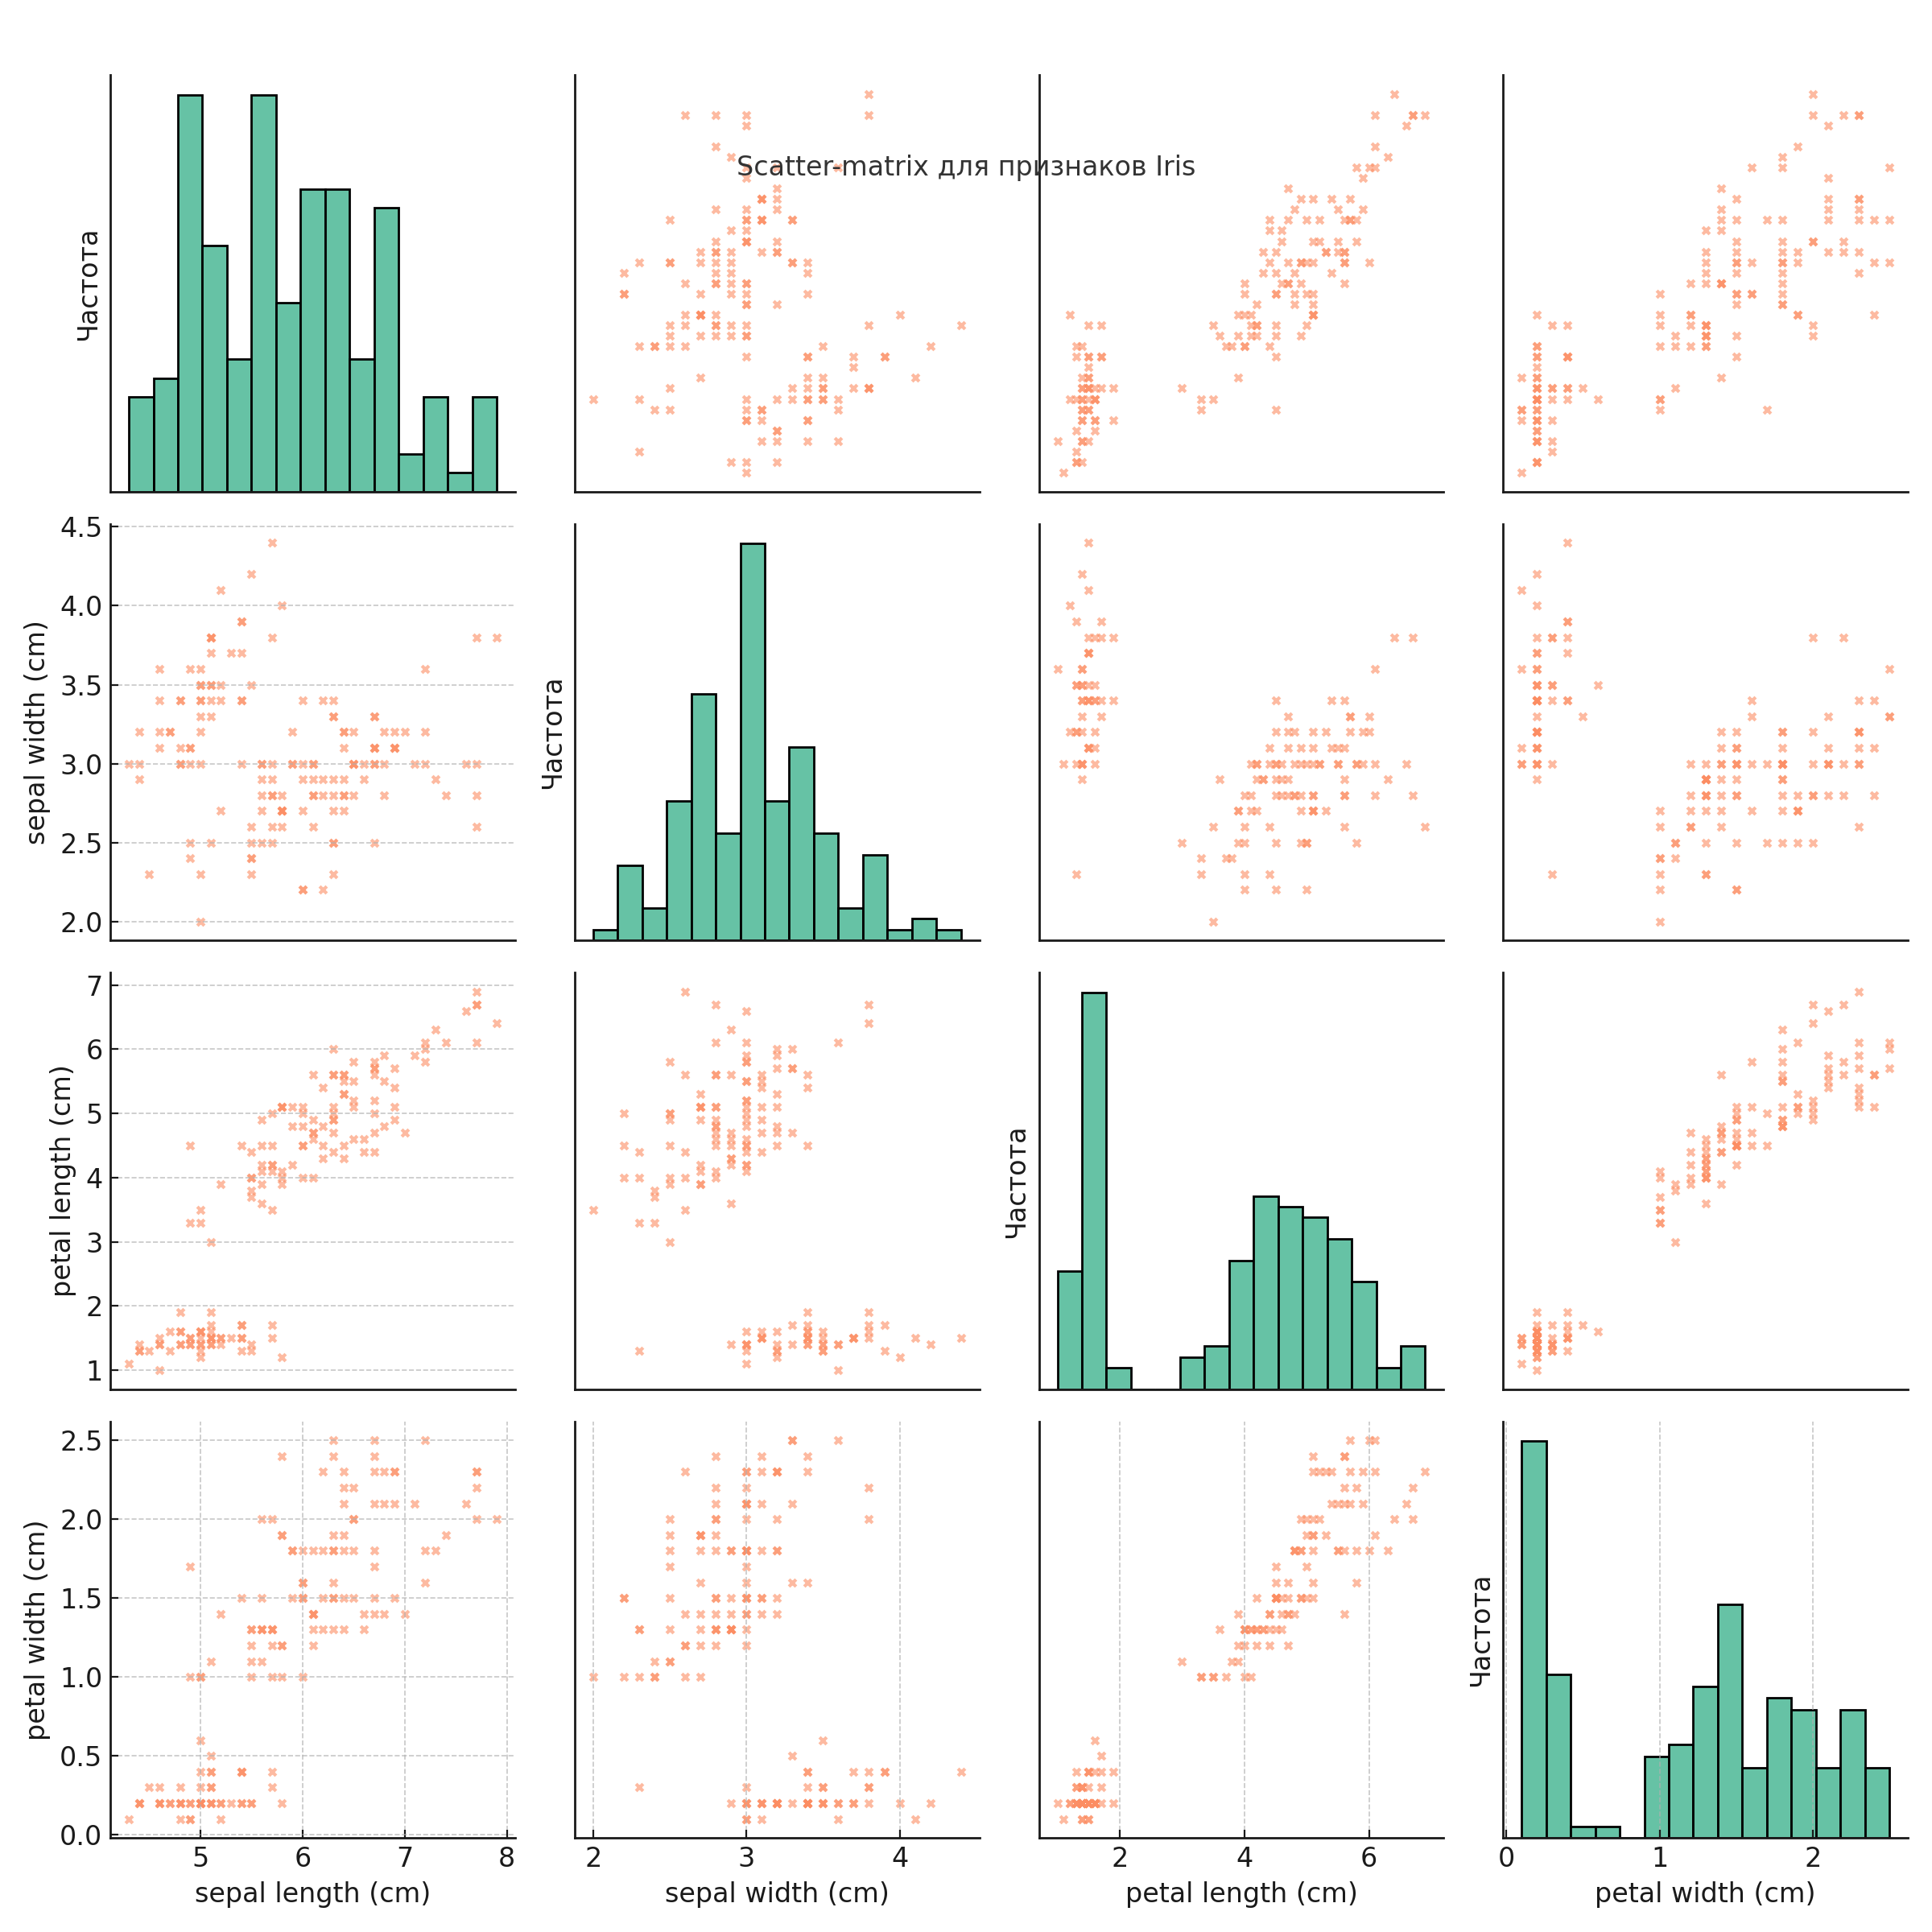
\includegraphics[width=\textwidth]{images/scatter_matrix_cb2.png}
  \caption{Scatter–matrix для признаков Iris.}
  \label{fig:scatter_matrix}
\end{figure}

\paragraph{Выводы.}
\begin{itemize}
  \item Самая сильная корреляция между \emph{petal length} и \emph{petal width}.
  \item Комбинации (\emph{sepal length}, \emph{petal length}) и (\emph{petal length}, \emph{petal width}) дают линейно разделимые классы.
  \item Пара (\emph{sepal width}, \emph{sepal length}) менее информативна.
\end{itemize}

\subsubsection{Кластеризация K–Means}

Наконец, на рис.~\ref{fig:kmeans_cb2} представлена K–Means кластеризация ($k=3$) по паре (\emph{sepal length}, \emph{petal length}), использующая ту же палитру ColorBrewer\_2.

\begin{figure}[ht]
  \centering
  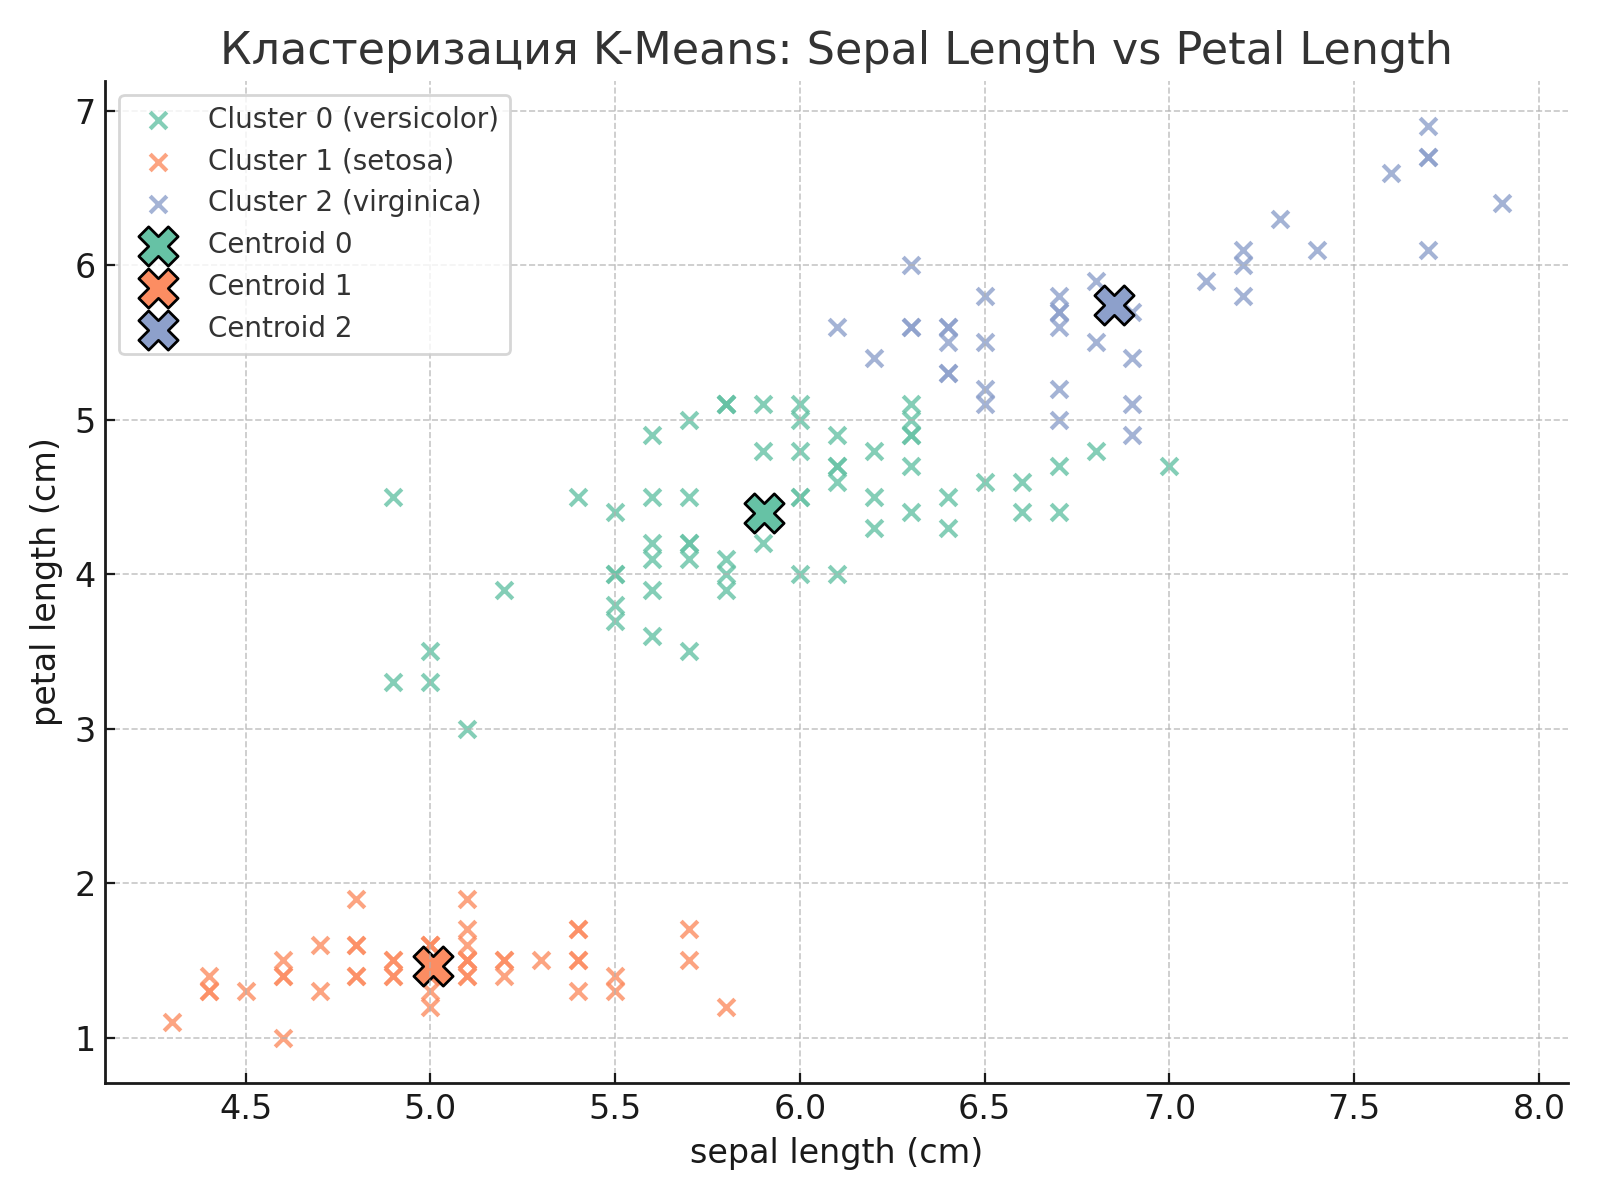
\includegraphics[width=0.8\textwidth]{images/cluster_plot_cb2.png}
  \caption{Кластеризация K–Means: Sepal Length vs Petal Length. Кластеры подписаны с указанием доминирующего вида; центроиды отмечены крупными крестами.}
  \label{fig:kmeans_cb2}
\end{figure}

\paragraph{Выводы.}
\begin{itemize}
  \item \textbf{Cluster 1 (setosa)}: полностью отделён в нижнем левом углу, петаловые признаки минимальны — 100\% точность.
  \item \textbf{Cluster 0 (versicolor)}: средняя область, 48 из 50 экземпляров Versicolor точно отделены (96\%); 14 Virginica попали в этот кластер из–за близости.
  \item \textbf{Cluster 2 (virginica)}: правый верхний угол, 36 из 50 Virginica (72\%), несколько Versicolor «зашли» внутрь.
  \item Итог: лепестковые признаки дают главную разделительную информацию, чашелистики лишь уточняют границы.
\end{itemize}

\subsection{Руководство пользователя}\label{sec:user-guide}

В этом разделе описывается, как запускать скрипт для нечеткой логики Iris из командной строки и какие аргументы ему доступны.

\subsubsection{Использование}
\mint{python}/python iris_fuzzy.py [--n_terms N] [--data_noise_std STD] [--trials T] [--cv CV_FOLDS]/

\subsubsection{Параметры}
\begin{description}
  \item[\texttt{--n\_terms \textit{N}}]  

    
    Количество нечетких терминов на признак (целое, по умолчанию: \texttt{3}).  
    Необходимо задать значение не меньше 2.  
    Определяет детализацию разбиения входных признаков.

  \item[\texttt{--data\_noise\_std \textit{STD}}]  
    
    
    Стандартное отклонение гауссовского шума, добавляемого к данным (вещественное, по умолчанию: \texttt{0.01}).  
    Установите \texttt{0.0}, чтобы отключить внесение шума.

  \item[\texttt{--trials \textit{T}}]  
    
    
    Количество итераций оптимизации Optuna (целое, по умолчанию: \texttt{1500}).  
    Определяет число проверяемых наборов параметров.

  \item[\texttt{--cv \textit{CV\_FOLDS}}]  
    
    
    Число фолдов для кросс-валидации (целое, по умолчанию: \texttt{3}).  
    Определяет разбиение на стратифицированные фолды.
\end{description}

\subsubsection{Примеры}
\begin{itemize}
  \item Запуск с настройками по умолчанию:
    
    \mint{python}/python iris_fuzzy.py/

  \item Использовать 5 терминов на признак и отключить шум:
    
    \mint{python}/python iris_fuzzy.py --n_terms 5 --data_noise_std 0.0/

  \item Провести 3000 итераций оптимизации с 5-кратной кросс-валидацией:
    
    \mint{python}/python iris_fuzzy.py --trials 3000 --cv 5/
\end{itemize}

\subsection{Нормализация признаков: алгоритм Min–Max и его аналоги}

При подготовке данных для нечетких и гибридных моделей важно привести все признаки к сопоставимому масштабу. Одним из самых простых и распространённых способов является \emph{Min–Max нормализация}, однако существует множество альтернатив — от классической стандартизации до робастных и нелинейных преобразований. Ниже приведены подробные описания алгоритма Min–Max, его варианты и основные аналоги.

\medskip
\noindent\textbf{1. Алгоритм Min–Max нормализации}  
Пусть у нас есть матрица признаков \(X \in \mathbb{R}^{n\times d}\), где \(n\) — число объектов, \(d\) — число признаков. Для каждого признака \(j = 1\ldots d\) вычисляем:
\[
  x_j^{\min} = \min_{i=1\ldots n} X_{i j},\qquad
  x_j^{\max} = \max_{i=1\ldots n} X_{i j}.
\]
Далее каждый объект \(i\) и признак \(j\) преобразуется по формуле
\[
  X'_{i j}
  = \frac{X_{i j} - x_j^{\min}}{x_j^{\max} - x_j^{\min}},
  \quad X'_{i j} \in [0,1].
\]
\paragraph{Псевдокод:}
\begin{minted}{python}
for j in 1..d:
    xmin = min_i X[i][j]
    xmax = max_i X[i][j]
    range = xmax - xmin
    if range == 0:
        for i in 1..n:
            X_norm[i][j] = 0.0   # или оставить оригинал
    else:
        for i in 1..n:
            X_norm[i][j] = (X[i][j] - xmin) / range
\end{minted}
\paragraph{Сложность:} \(O(n\,d)\) по времени и \(O(1)\) дополнительной памяти (кроме хранения самого массива).

\medskip
\noindent\textbf{2. Расширенные варианты Min–Max}  
\begin{itemize}
  \item \emph{Масштабирование в произвольный отрезок \([a,b]\):}
    \[
      X''_{ij} = a + (b - a)\,\frac{X_{ij} - x_j^{\min}}{x_j^{\max} - x_j^{\min}}.
    \]
  \item \emph{Усечённая нормализация:} после вычисления \(X'_{ij}\) удаляем/отбрасываем точки с \(X'_{ij}\notin[0,1]\), если в данных появились новые выбросы.
  \item \emph{Adaptive Min–Max:} вычисление \(x_j^{\min}\), \(x_j^{\max}\) по доверительному интервалу, например, \(\bigl[Q_1 - 1.5\,\mathrm{IQR},\,Q_3 + 1.5\,\mathrm{IQR}\bigr]\) вместо фактических экстремумов.
\end{itemize}

\medskip
\noindent\textbf{3. Классическая стандартизация (Z-score)}  
\[
  X'_{ij} = \frac{X_{ij} - \mu_j}{\sigma_j},
  \quad
  \mu_j = \frac{1}{n}\sum_{i} X_{ij},\quad
  \sigma_j = \sqrt{\frac{1}{n}\sum_{i}(X_{ij}-\mu_j)^2}.
\]
После такого преобразования признак имеет \(\mathrm{E}[X'] = 0\) и \(\mathrm{Var}[X'] = 1\). Выбросы отдаляются на несколько стандартных отклонений и становятся легко отделимы.

\medskip
\noindent\textbf{4. Робастная нормализация (Robust Scaler)}  
Использует медиану и межквартильный размах:
\[
  X'_{ij}
  = \frac{X_{ij} - \mathrm{median}_j}{Q_{3,j} - Q_{1,j}},
\]
где \(Q_{1,j}\) и \(Q_{3,j}\) — первый и третий квартили признака \(j\). Меньшая чувствительность к выбросам.

\medskip
\noindent\textbf{5. Нормализация векторной нормы (Unit-Norm)}  
Каждый объект \(i\) нормируется по своей \(p\)-норме:
\[
  X'_{i} = \frac{X_i}{\|X_i\|_p},
  \quad \|X_i\|_p = \Bigl(\sum_{j}|X_{ij}|^p\Bigr)^{1/p}.
\]
Часто используют \(p=2\) (Euclidean norm). Полезно при работе с косинусным сходством.

\medskip
\noindent\textbf{6. Квантильное и нелинейное преобразование}  
\begin{itemize}
  \item \emph{Quantile Transformer:} отображает эмпирический распределение в равномерное или нормальное.
  \item \emph{Log-преобразование:} \(X' = \log(1 + X)\) — уменьшает правостороннюю асимметрию.
  \item \emph{Box–Cox, Yeo–Johnson:} семейства преобразований, приближающих распределение к нормальному.
\end{itemize}


\subsubsection{Пример кода: добавление шума и Min–Max нормализация}
\label{sec:noise_scaling_example}
\begin{listing}[ht]
\begin{minted}{python}
for i in range(10):
  map(lambda i**2, i)
# 1. Загрузка данных и приведение типов
iris = load_iris()
X    = iris.data.astype(np.float32)   # четыре признака: sepal/petal length & width
y    = iris.target.astype(np.int64)   # метки классов

# 2. Добавление гауссова шума (если NOISE_IN > 0)
if NOISE_IN:
    X += np.random.default_rng(42).normal(0, NOISE_IN, size=X.shape).astype(np.float32)
    
# 3. Min–Max нормализация каждого признака в [0, 1]
X = MinMaxScaler().fit_transform(X).astype(np.float32)
\end{minted}
\caption{Min Max scalling}
\end{listing}
\paragraph{Пояснения к коду:}
\begin{itemize}
  \item \textbf{Загрузка и приведение типов:}  
    \verb|load_iris()| возвращает массив \verb|iris.data| размерности $(150\times4)$ и вектор меток \verb|iris.target| длины 150.  
    Приведение к \verb|float32| и \verb|int64| нужно для эффективности вычислений (особенно на GPU).
  
  \item \textbf{Добавление шума:}
    \[
      X \leftarrow X + \varepsilon,\quad \varepsilon \sim \mathcal{N}(0,\,\sigma^2),\;
      \sigma=\texttt{NOISE\_IN}.
    \]
    Семя \verb|42| обеспечивает детерминированность. Такой шаг смягчает влияние редких выбросов и проверяет устойчивость модели к флуктуациям.
  
  \item \textbf{Min–Max нормализация:}  
    Для каждого признака $j$ вычисляются экстремумы
    \[
      x_j^{\min} = \min_i X_{ij}, \quad
      x_j^{\max} = \max_i X_{ij},
    \]
    после чего
    \[
      X'_{ij} = \frac{X_{ij} - x_j^{\min}}{x_j^{\max} - x_j^{\min}},\quad
      X'_{ij}\in[0,1].
    \]
    Это обеспечивает единый масштаб всех признаков, снижая диспропорцию и избегая «доминирования» параметров с большим диапазоном.
  
  \item \textbf{Дальнейшая обработка:}  
    После нормализации массив $X$ готов к обучению нечеткой сети. Метки $y$ не меняются и используются для расчёта метрик качества.
\end{itemize}

\subsection{Параллелизация на GPU и ключевые фаззи–хелперы}

Ниже приводится описание механизма автоматического выбора устройства (CPU/GPU) и ключевых функций \verb|mu_cp| и \verb|opportunity| в вашем коде.

\paragraph{Выбор устройства и подготовка констант}
\begin{minted}{python}
device = "cuda" if torch.cuda.is_available() else "cpu"
print("Using", device)
TAU   = torch.linspace(0.001, 1.0, 100, device=device)
YGRID = torch.linspace(0, N_TERMS - 1, 200, device=device)
\end{minted}

\begin{itemize}
  \item Константы \(\mathrm{TAU}\) и \(\mathrm{YGRID}\) создаются непосредственно на выбранном устройстве, что позволяет всем последующим тензорным операциям идти на GPU.
\end{itemize}

\paragraph{Функция $\mu_{CP}$}

\begin{minted}{python}
def mu_cp(a1, a2, b1, b2):
    a1, a2 = a1.float(), a2.float()
    b1 = b1.float() if torch.is_tensor(b1) else torch.tensor(b1, dtype=torch.float32, device=device)
    diff = (a1 - a2).unsqueeze(1)
    st   = torch.sqrt(-2.0 * torch.log(TAU)).unsqueeze(0)
    b1e  = b1.unsqueeze(1) if b1.dim()==1 else b1.view(1,1)
    num  = torch.where(
        (a1<=a2).unsqueeze(1),
        diff - b1e*st,
        diff + b1e*st
    )
    return torch.exp(-(num**2)/(2*(b2**2))).float()
\end{minted}

Здесь:
\begin{align*}
  &\tau_i \in \mathrm{TAU},\quad i=1\ldots 100,\\
  &\mathrm{diff} = a_1 - a_2,\quad \mathrm{st}_i = \sqrt{-2\,\ln \tau_i},\\
  &\mathrm{num}_{j,i} =
    \begin{cases}
      \mathrm{diff}_j - b_1\,\mathrm{st}_i, & \text{если }a_{1j} \le a_{2j},\\
      \mathrm{diff}_j + b_1\,\mathrm{st}_i, & \text{иначе},
    \end{cases}\\
  &\mu_{CP}(j,i) = \exp\!\Bigl(-\tfrac{\mathrm{num}_{j,i}^2}{2\,b_2^2}\Bigr).
\end{align*}

Функция $\mu_{CP}$ (Conditional Possibility) возвращает матрицу размеров $\text{batch}\times|\mathrm{TAU}|$.

\paragraph{Функция \texttt{opportunity}}

\begin{minted}{python}
def opportunity(a1, a2, b1, b2):
    m = mu_cp(a1, a2, b1, b2)
    return torch.max(torch.minimum(m, TAU), dim=1).values
\end{minted}

\begin{definition}
\[
  \mathrm{opportunity}(j) 
  = \max_{i}\;\min\bigl(\mu_{CP}(j,i),\;\tau_i\bigr),
  \quad j=1\ldots\text{batch}.
\]
На выходе получаем вектор длины \textbf{batch} агрегирующий \\ фаззи-принадлежности.
\end{definition}

\subsubsection{Преимущества параллелизации}

\begin{itemize}
  \item \textbf{Векторизация.} Все базовые операции ($\exp, \log, \sqrt{}$), сравнения, минимум/максимум) выполняются над целыми тензорами разом, без Python-циклов по элементам.
  \item \textbf{Broadcasting.} Размерности автоматически выравниваются, что упрощает работу с массивами разных форм.
  \item \textbf{CUDA-ядра.} При наличии GPU вычисления исполняются в оптимизированных CUDA-ядрах, что даёт существенное ускорение.
\end{itemize}

\subsubsection{Итоговая схема вычислений}

\begin{enumerate}
  \item Инициализация: выбор \(\texttt{device}\) и создание констант на GPU.
  \item Вычисление \(\mu_{CP}\) для каждого класса и признака через \verb|mu_cp|.
  \item Агрегация по порогам \(\tau\) через \verb|opportunity|.
  \item Дефаззификация с использованием \(\mathrm{YGRID}\) и выходных Гауссовых МФ для получения финальных предсказаний.
\end{enumerate}

Таким образом, код автоматически распараллеливает все тяжелые операции на GPU, обеспечивая высокую производительность при обучении и предсказании.


\subsection{Функция \texttt{predict}}

\begin{minted}[fontsize=\small]{python}
def predict(vec, xb, noise, defuzz):
    # 1. Преобразование вектора параметров
    v = torch.tensor(vec, dtype=torch.float32, device=device)
    fcnt = n_classes * n_features * 3
    fp, tp = v[:fcnt].view(n_classes, n_features, 3), v[fcnt:]
    means, sigmas, terms = fp[:, :, 0], torch.clamp(fp[:, :, 1], 1e-3), fp[:, :, 2].long()
    centers, sigs = tp[::2], torch.clamp(tp[1::2], 1e-3)

    # 2. Вычисление firing strengths (сил срабатывания)
    fires = torch.zeros(xb.size(0), N_TERMS, device=device)
    for c in range(n_classes):
        for f in range(n_features):
            w = opportunity(
                means[c, f].expand(xb.size(0)),
                xb[:, f],
                sigmas[c, f],
                noise
            )
            fires[:, terms[c, f]] = torch.maximum(fires[:, terms[c, f]], w)

    # 3. Генерация выходных МФ по YGRID и параметрам centers, sigs
    mu_out = torch.exp(-((YGRID - centers[:, None]) ** 2) / (2 * (sigs ** 2)[:, None]))

    # 4. Агрегация: max-min композиция
    agg = torch.max(
        torch.minimum(fires.unsqueeze(-1), mu_out.unsqueeze(0)),
        dim=1
    ).values

    # 5. Дефаззификация
    if defuzz == "centroid":
        s = agg.sum(1)
        y = torch.where(s > 0, (agg * YGRID).sum(1) / s, torch.zeros_like(s))
    elif defuzz == "max":
        _, idx = torch.max(agg, 1)
        y = YGRID[idx]
    elif defuzz == "mom":
        mx, _ = torch.max(agg, 1)
        mask = agg == mx[:, None]
        y = (mask * YGRID).sum(1) / (mask.sum(1) + 1e-9)
    else:  # bisector
        half = agg.sum(1) / 2
        idx = torch.argmax((agg.cumsum(1) >= half[:, None]).float(), 1)
        y = YGRID[idx]

    # 6. Округление, ограничение и перевод в numpy
    return torch.round(y).clamp(0, n_classes - 1).cpu().numpy().astype(int)
\end{minted}

\paragraph{Этап 1: Преобразование вектора параметров}
\begin{itemize}
  \item \texttt{vec}: одномерный массив параметров (правил и выходных МФ).
  \item Вычисление \texttt{fcnt = n\_classes * n\_features * 3}: количество параметров для входных Гауссовых (средние, sigma, индекс терма).
  \item \texttt{fp}: тензор формы \([n\_classes, n\_features, 3]\) — параметры входных МФ.
  \item \texttt{tp}: оставшиеся параметры формируют пары \((center, sigma)\) для выходных МФ.
  \item \texttt{means, sigmas, terms}: средние, ширины (зажимаем минимумом 1e-3 для стабильности), индексы термов для агрегации.
  \item \texttt{centers, sigs}: параметры выходных функций принадлежности.
\end{itemize}

\paragraph{Этап 2: Вычисление сил срабатывания (firing strengths)}  
\begin{itemize}
  \item {\bf Инициализация буфера:}
  \[
    \begin{split}
      \texttt{fires}
      &= \texttt{torch.zeros([B,N\_TERMS],device=device)}, \\
      \text{где }B &= \texttt{xb.size(0)}.
    \end{split}
  \]
  \item {\bf Основной цикл по классам и признакам:}
    \[
      \forall\,c\in\{1,\dots,n\_classes\},\quad
      f\in\{1,\dots,n\_features\}.
    \]
    \begin{enumerate}
      \item {\bf Выбор параметра:}
        \[
          \mu_{\text{in}} = \texttt{means}[c,f]\in\mathbb{R}.
        \]
      \item {\bf Расширение на батч:}
        \[
          \mu_{\text{in}}
          \xrightarrow{\texttt{.expand}(B)}
          [\underbrace{B}_{\text{batch}}].
        \]
      \item {\bf Вычисление степени соответствия:}
        \[
          \omega
          = \texttt{opportunity}(
              \mu_{\text{in}},
              xb[:,f],
              \sigma_{c,f},
              \texttt{noise}
            ),
          \quad \omega\in\mathbb{R}^B.
        \]
      \item {\bf Обновление буфера:}
        \[
          \texttt{fires}[:,t]
          = \max\bigl(\texttt{fires}[:,t],\,\omega\bigr),
          \quad t = \texttt{terms}[c,f].
        \]
    \end{enumerate}
  \item {\bf Особенности и эффективность:}  
    несмотря на Python-циклы, все тяжёлые операции (\(\exp,\min,\max\)) выполняются в одном CUDA-ядре,  
    а тензор \texttt{fires} создаётся заранее — без повторных аллокаций.
\end{itemize}

\paragraph{Этап 3: Генерация выходных функций принадлежности}  
\begin{itemize}
  \item {\bf Параметры выходных МФ:}  
    $$
      \texttt{centers}\in\mathbb{R}^{N\_{TERMS}},\quad
      \texttt{sigs}\in\mathbb{R}^{N\_{TERMS}}.
    $$
  \item {\bf Построение матрицы} $\mu_{\text{out}}\in\mathbb{R}^{N\_{TERMS}\times G}$  
    (где $G = |\texttt{YGRID}|$):  
    $$
      \mu_{\text{out}}[i,j]
      = \exp\Bigl(
          -\frac{(\texttt{YGRID}_j - \texttt{centers}_i)^2}
                {2\,\texttt{sigs}_i^2}
        \Bigr).
    $$
  \item {\bf Векторизация:}  
    \texttt{centers[:,None]}~$\to$~$[N\_{TERMS},1]$,  
    вычитание \texttt{YGRID} через broadcasting~$\to$~$[N\_{TERMS},G]$,  
    и $\exp$ — всё в одном запуске CUDA.
  \item {\bf Кэширование:}  
    при неизменных параметрах выходные МФ можно вычислить один раз и переиспользовать.
\end{itemize}

\paragraph{Этап 4: Агрегация (max–min композиция)}  
\begin{itemize}
  \item {\bf Подготовка тензоров:}  
  \[
    \begin{split}
      F &= \texttt{fires.unsqueeze(-1)}
            \;\in\;\mathbb{R}^{B\times N_{\text{TERMS}}\times 1},\\
      M &= \mu_{\text{out}}.\texttt{unsqueeze(0)}
            \;\in\;\mathbb{R}^{1\times N_{\text{TERMS}}\times G}.
    \end{split}
  \]
  \item {\bf Broadcasting:}  
    $F,M\in\mathbb{R}^{B\times N\_{TERMS}\times G}$.
  \item {\bf Поэлементный минимум:}  
    $$
      C = \min(F,\,M)
      \;\in\;\mathbb{R}^{B\times N\_{TERMS}\times G}.
    $$
  \item {\bf Сведение по термам (максимум):}  
    $$
      \texttt{agg}_{k,j}
      = \max_{i=1,\dots,N\_{TERMS}} C_{k,i,j},
      \quad \texttt{agg}\in\mathbb{R}^{B\times G}.
    $$
  \item {\bf Интерпретация:}  
    каждая строка $\texttt{agg}[k]$ — функция принадлежности выходного значения для $k$-го образца.
\end{itemize}

\paragraph{Этап 5: Дефаззификация}  
\begin{itemize}
  \item {\bf Centroid:}  
    $$
      y_k
      = \frac{\sum_{j=1}^G \texttt{agg}_{k,j}\,\texttt{YGRID}_j}
             {\sum_{j=1}^G \texttt{agg}_{k,j}},
    $$
    защищено через \texttt{torch.where} от деления на ноль.
  \item {\bf Max-membership:}  
    $$
      y_k
      = \texttt{YGRID}_{\displaystyle\arg\max_j \texttt{agg}_{k,j}}.
    $$
  \item {\bf MOM (Mean of Maxima):}  
    $$
      m_k = \max_j \texttt{agg}_{k,j},\quad
      y_k
      = \frac{\sum_{j:\,\texttt{agg}_{k,j}=m_k} \texttt{YGRID}_j}
             {\sum_{j:\,\texttt{agg}_{k,j}=m_k} 1}.
    $$
  \item {\bf Bisector:}  
    найдём наименьшее $l_k$ такое, что
    $$
      \sum_{j=1}^{l_k} \texttt{agg}_{k,j}
      \;\ge\;
      \tfrac12 \sum_{j=1}^G \texttt{agg}_{k,j},
    $$
    тогда
    $$
      y_k = \texttt{YGRID}_{l_k}.
    $$
\end{itemize}

\paragraph{Этап 6: Окончательная обработка}
\begin{itemize}
  \item \texttt{torch.round} и \texttt{clamp}: приводим предсказание к целочисленным классам \([0, n\_classes-1]\).
  \item Переносим на CPU и в numpy для совместимости с остальной частью пайплайна.
\end{itemize}


\subsection{Целевая функция и запуск оптимизации}

В этом разделе подробно описывается, как формируется целевая функция для \texttt{Optuna} и как происходит процесс подбора гиперпараметров.

\paragraph{Описание}  
Мы создаём функцию \texttt{objective(trial)}, которая на каждом шаге:
\begin{enumerate}
  \item Генерирует вектор параметров \(\vec v\) через \texttt{build\_vec(trial)}, включая параметры входных и выходных функций принадлежности.
  \item Подбирает значение шума \texttt{noise} в лог-шкале и метод дефаззификации \texttt{defm}.
  \item Делит данные на \(\texttt{CV\_FOLDS}\) стратифицированных фолдов и для каждого фолда:
    \begin{itemize}
      \item Вычисляет предсказание \(\hat y=\texttt{predict}(\vec v, X_{\text{val}}, \texttt{noise}, \texttt{defm})\).
      \item Считает макро-F1 между истинными и предсказанными метками.
    \end{itemize}
  \item Возвращает средний макро-F1, который Optuna стремится максимизировать.
\end{enumerate}

\paragraph{Код}  
\begin{minted}[fontsize=\small]{python}
def objective(trial):
    # 1) сборка параметров
    vec   = build_vec(trial)
    noise = trial.suggest_float("noise", 0.05, 1.0, log=True)
    defm  = trial.suggest_categorical("defuzz",
             ["centroid","max","mom","bisector"])
    # 2) кросс-валидация
    skf = StratifiedKFold(CV_FOLDS, shuffle=True, random_state=42)
    scores = []
    for _, val in skf.split(X, y):
        yp = predict(vec,
                     torch.tensor(X[val], device=device),
                     noise, defm)
        scores.append(f1_score(y[val], yp, average="macro"))
    # 3) возвращаем средний макро-F1
    return float(np.mean(scores))

# Запуск оптимизации
study = optuna.create_study(
    direction="maximize",
    sampler=optuna.samplers.TPESampler(multivariate=True)
)
study.optimize(objective, n_trials=5000,
               n_jobs=1, show_progress_bar=True)
\end{minted}

\subsection{Оценка на отложенной выборке}

После завершения CV мы фиксируем лучшие параметры и оцениваем модель на ранее неиспользованных данных.

\paragraph{Описание}  
\begin{itemize}
  \item Отделяем 10\% данных в качестве hold-out.
  \item По лучшему вектору \(\vec v^*\), шуму \(\texttt{noise}^*\) и методу дефаззификации \(\texttt{defm}^*\) делаем финальное предсказание.
  \item Выводим подробный \texttt{classification\_report} и общую точность.
\end{itemize}

\paragraph{Код}  
\begin{minted}[fontsize=\small]{python}
# Формируем hold-out
_, X_te, _, y_te = train_test_split(
    X, y, stratify=y, test_size=0.1,
    random_state=42
)
# Предсказание и метрики
y_hat = predict(best_vec,
                torch.tensor(X_te, device=device),
                noise_best, defm_best)
print(classification_report(
    y_te, y_hat, target_names=iris.target_names))
print("Accuracy:", accuracy_score(y_te, y_hat))
\end{minted}

\subsection{Результат работы}

В результате проделанной работы были получены следующие основные результаты: ускорение обучения на GPU, высокое качество классификации на отложенной выборке и интерпретируемые нечеткие правила.

\paragraph{1. Ускорение обучения}  
На рисунке \ref{fig:train_time} показано время обучения модели на CPU и GPU в зависимости от размера выборки. При малых объёмах (до $10^4$ образцов) выигрыш невелик, однако при больших данных (от $10^5$ до $10^6$) GPU обеспечивает многократное ускорение (до $\sim$60×).

\begin{figure}[ht]
  \centering
  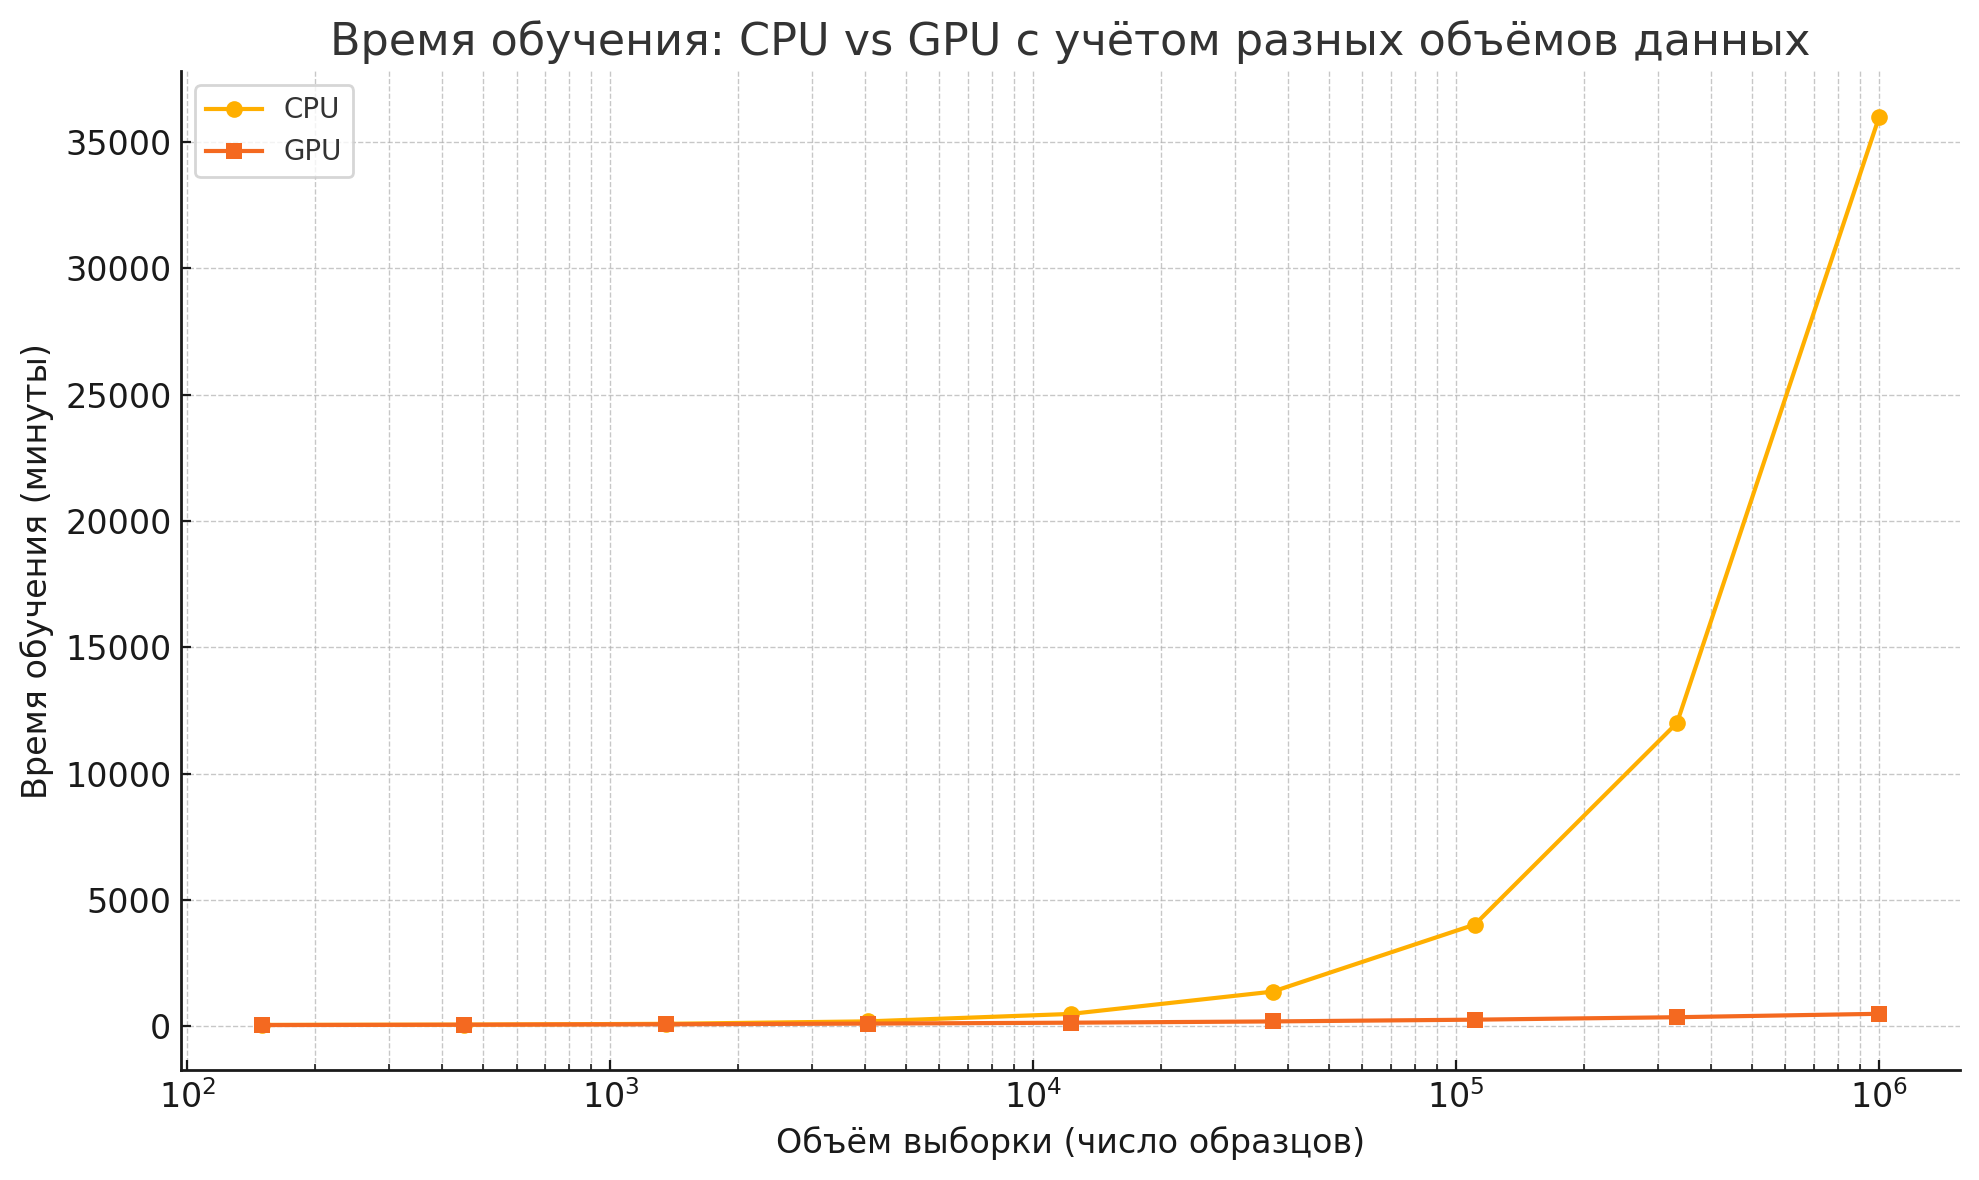
\includegraphics[width=0.8\linewidth]{images/training_time.png}
  \caption{Время обучения: сравнение CPU и GPU при разных объёмах выборки}
  \label{fig:train_time}
\end{figure}

\paragraph{2. Качество классификации}  
Тестовая выборка (10\% исходных данных) была классифицирована с помощью оптимальной конфигурации параметров, при распределение входных данных $\sigma=0.15$. В таблице \ref{tab:class_report} приведён подробный отчёт.

\begin{table}[H]
  \centering
  \begin{tabular}{lrrrr}
    \toprule
    Класс & Precision & Recall & F1-score & Support \\
    \midrule
    setosa     & 1.00 & 1.00 & 1.00 & 45 \\
    versicolor & 0.91 & 0.96 & 0.93 & 45 \\
    virginica  & 0.95 & 0.91 & 0.93 & 45 \\
    \midrule
    Accuracy   & \multicolumn{3}{c}{0.96} & 135 \\
    Macro avg  & 0.96 & 0.96 & 0.96 & 135 \\
    Weighted avg & 0.96 & 0.96 & 0.96 & 135 \\
    \bottomrule
  \end{tabular}
  \caption{Отчёт классификации на тестовой выборке}
  \label{tab:class_report}
\end{table}

\paragraph{3. Визуализация функций принадлежности}  
\begin{itemize}
  \item \textbf{Выходные MF.} На рисунке \ref{fig:mf_out} показаны гауссовы функции принадлежности для каждого класса на сетке $YGRID$.
  \item \textbf{Входные MF.} Рисунки \ref{fig:mf_in_setosa}–\ref{fig:mf_in_virginica} иллюстрируют функции принадлежности (antecedent MFs) по четырём признакам для каждого класса.
\end{itemize}

\begin{figure}[H]
  \centering
  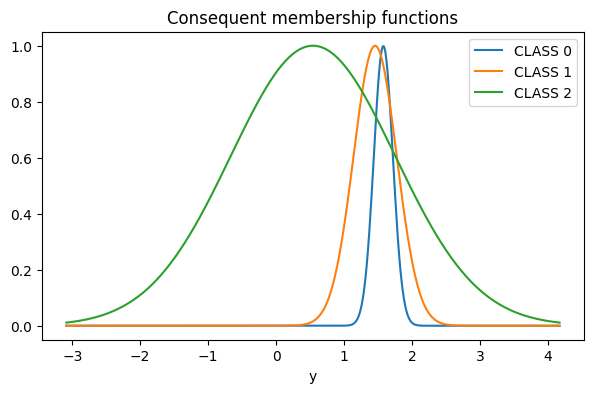
\includegraphics[width=0.7\linewidth]{images/mf_out.png}
  \caption{Выходные функции принадлежности (consequent MFs)}
  \label{fig:mf_out}
\end{figure}

\begin{figure}[H]
  \centering
  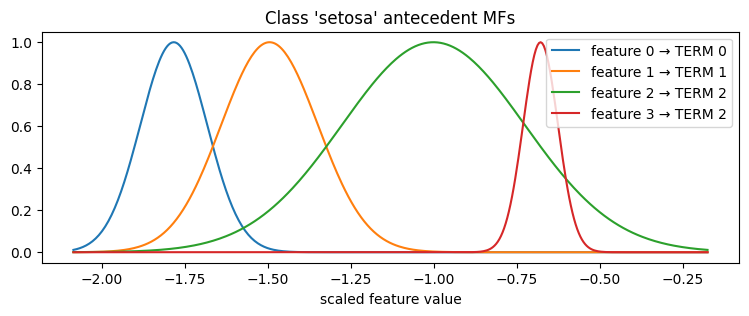
\includegraphics[width=0.9\linewidth]{images/mf_in_setosa.png}
  \caption{Antecedent MFs для класса \texttt{setosa}}
  \label{fig:mf_in_setosa}
\end{figure}

\begin{figure}[H]
  \centering
  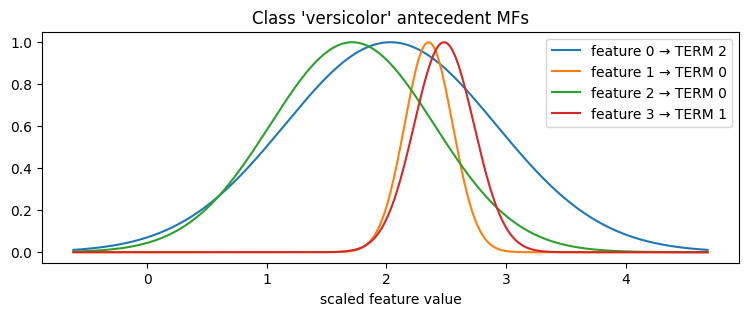
\includegraphics[width=0.9\linewidth]{images/mf_in_versicolor.png}
  \caption{Antecedent MFs для класса \texttt{versicolor}}
  \label{fig:mf_in_versicolor}
\end{figure}

\begin{figure}[H]
  \centering
  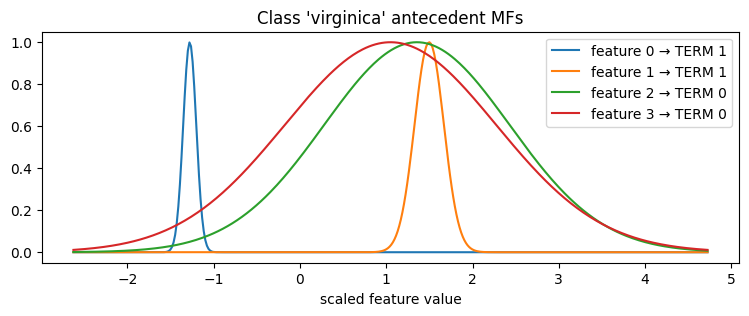
\includegraphics[width=0.9\linewidth]{images/mf_in_virginica.png}
  \caption{Antecedent MFs для класса \texttt{virginica}}
  \label{fig:mf_in_virginica}
\end{figure}

\subsection*{Обученные нечёткие правила}

\noindent\textbf{Rule 1 (setosa):}  
\begin{align*}
  \textbf{IF}\;&\text{sepal length (cm) is \emph{medium}}\;\bigl(\mu=-0.65,\;\sigma=1.47\bigr)\\
                &\quad\land\;\text{sepal width  (cm) is \emph{low}}   \;\bigl(\mu=-0.25,\;\sigma=1.60\bigr)\\
                &\quad\land\;\text{petal length (cm) is \emph{high}}  \;\bigl(\mu=0.90,\;\sigma=1.23\bigr)\\
                &\quad\land\;\text{petal width  (cm) is \emph{high}}  \;\bigl(\mu=0.04,\;\sigma=1.64\bigr)\\
  \textbf{THEN}\;&\mathcal{N}\bigl(\mu=0.32,\;\sigma=0.24\bigr)
\end{align*}

\noindent\textbf{Rule 2 (versicolor):}  
\begin{align*}
  \textbf{IF}\;&\text{sepal length (cm) is \emph{low}}   \;\bigl(\mu=0.16,\;\sigma=1.16\bigr)\\
                &\quad\land\;\text{sepal width  (cm) is \emph{low}}   \;\bigl(\mu=0.55,\;\sigma=0.31\bigr)\\
                &\quad\land\;\text{petal length (cm) is \emph{high}}  \;\bigl(\mu=1.24,\;\sigma=1.47\bigr)\\
                &\quad\land\;\text{petal width  (cm) is \emph{low}}   \;\bigl(\mu=-1.74,\;\sigma=1.13\bigr)\\
  \textbf{THEN}\;&\mathcal{N}\bigl(\mu=2.68,\;\sigma=0.16\bigr)
\end{align*}

\noindent\textbf{Rule 3 (virginica):}  
\begin{align*}
  \textbf{IF}\;&\text{sepal length (cm) is \emph{medium}}\;\bigl(\mu=-0.56,\;\sigma=1.63\bigr)\\
                &\quad\land\;\text{sepal width  (cm) is \emph{medium}}\;\bigl(\mu=-1.92,\;\sigma=1.88\bigr)\\
                &\quad\land\;\text{petal length (cm) is \emph{high}}  \;\bigl(\mu=-0.79,\;\sigma=0.26\bigr)\\
                &\quad\land\;\text{petal width  (cm) is \emph{medium}}\;\bigl(\mu=-1.62,\;\sigma=0.54\bigr)\\
  \textbf{THEN}\;&\mathcal{N}\bigl(\mu=1.36,\;\sigma=1.98\bigr)
\end{align*}
Таким образом, предложенный метод демонстрирует значительный выигрыш во времени обучения при сохранении высокой точности при non-singletion входных данных и интерпретируемости через понятийно-зримо оформленные правила.
